\documentclass{article}
\usepackage{graphicx}

\title{RESUME VIDEO ORACLE}
\author{Gany Berdu Sura}

\date{1184008}

\begin{document}

\maketitle

\section{Oracle APEX}
\begin{enumerate}
\item Buka oracleapex.com
\begin{figure}[h]
\centerline{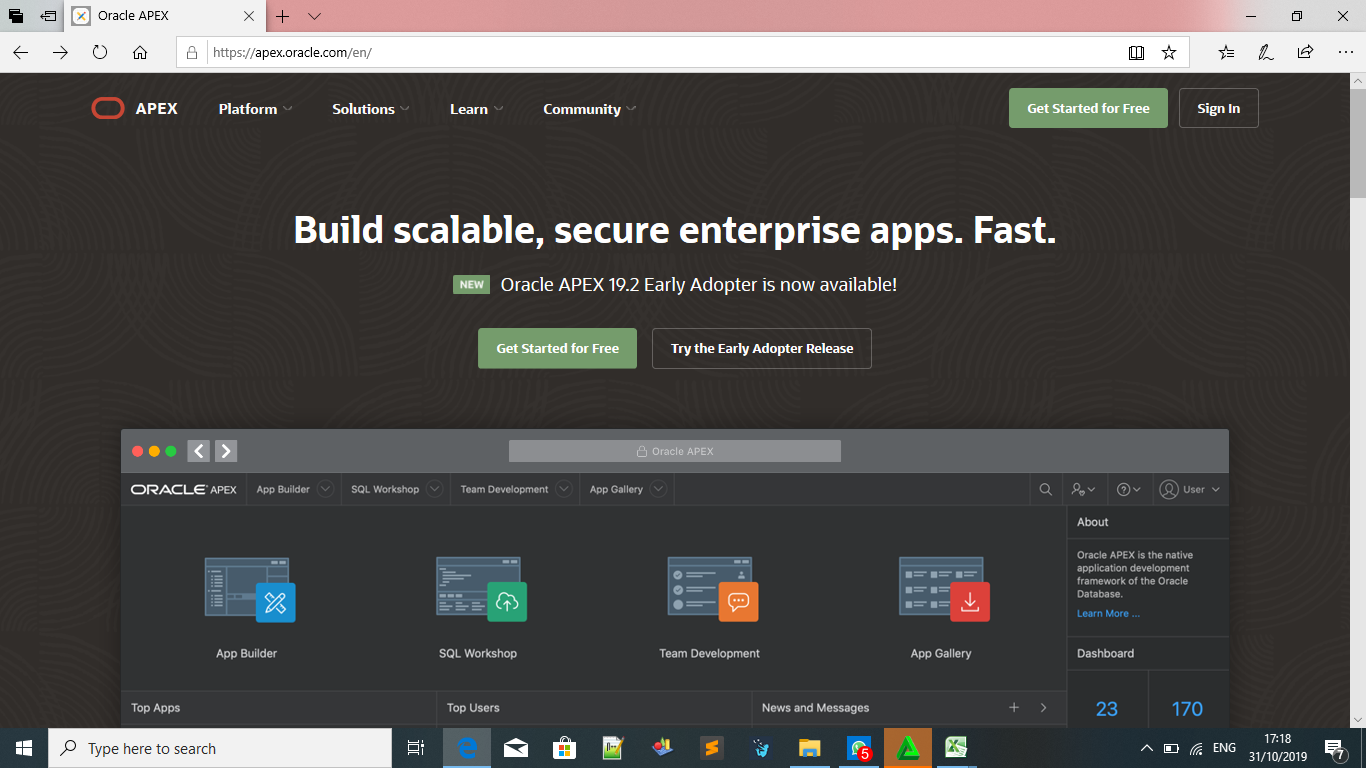
\includegraphics[width=8cm]{figure/sa.png}}
            \end{figure}
            \item isi workspace,username,dan password
\begin{figure}[h]
\centerline{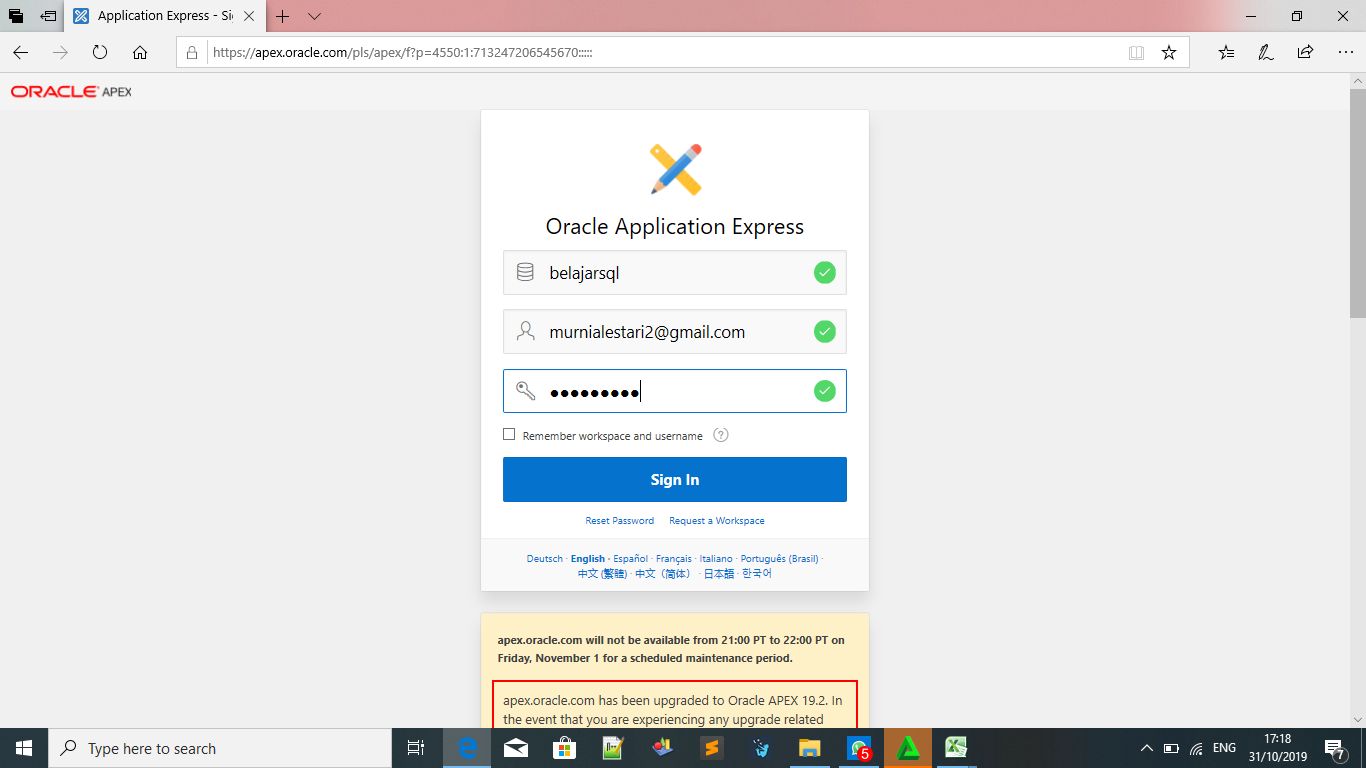
\includegraphics[width=8cm]{figure/su.png}}
            \end{figure}
\newpage\item Pilih app builder
\begin{figure}[h]
\centerline{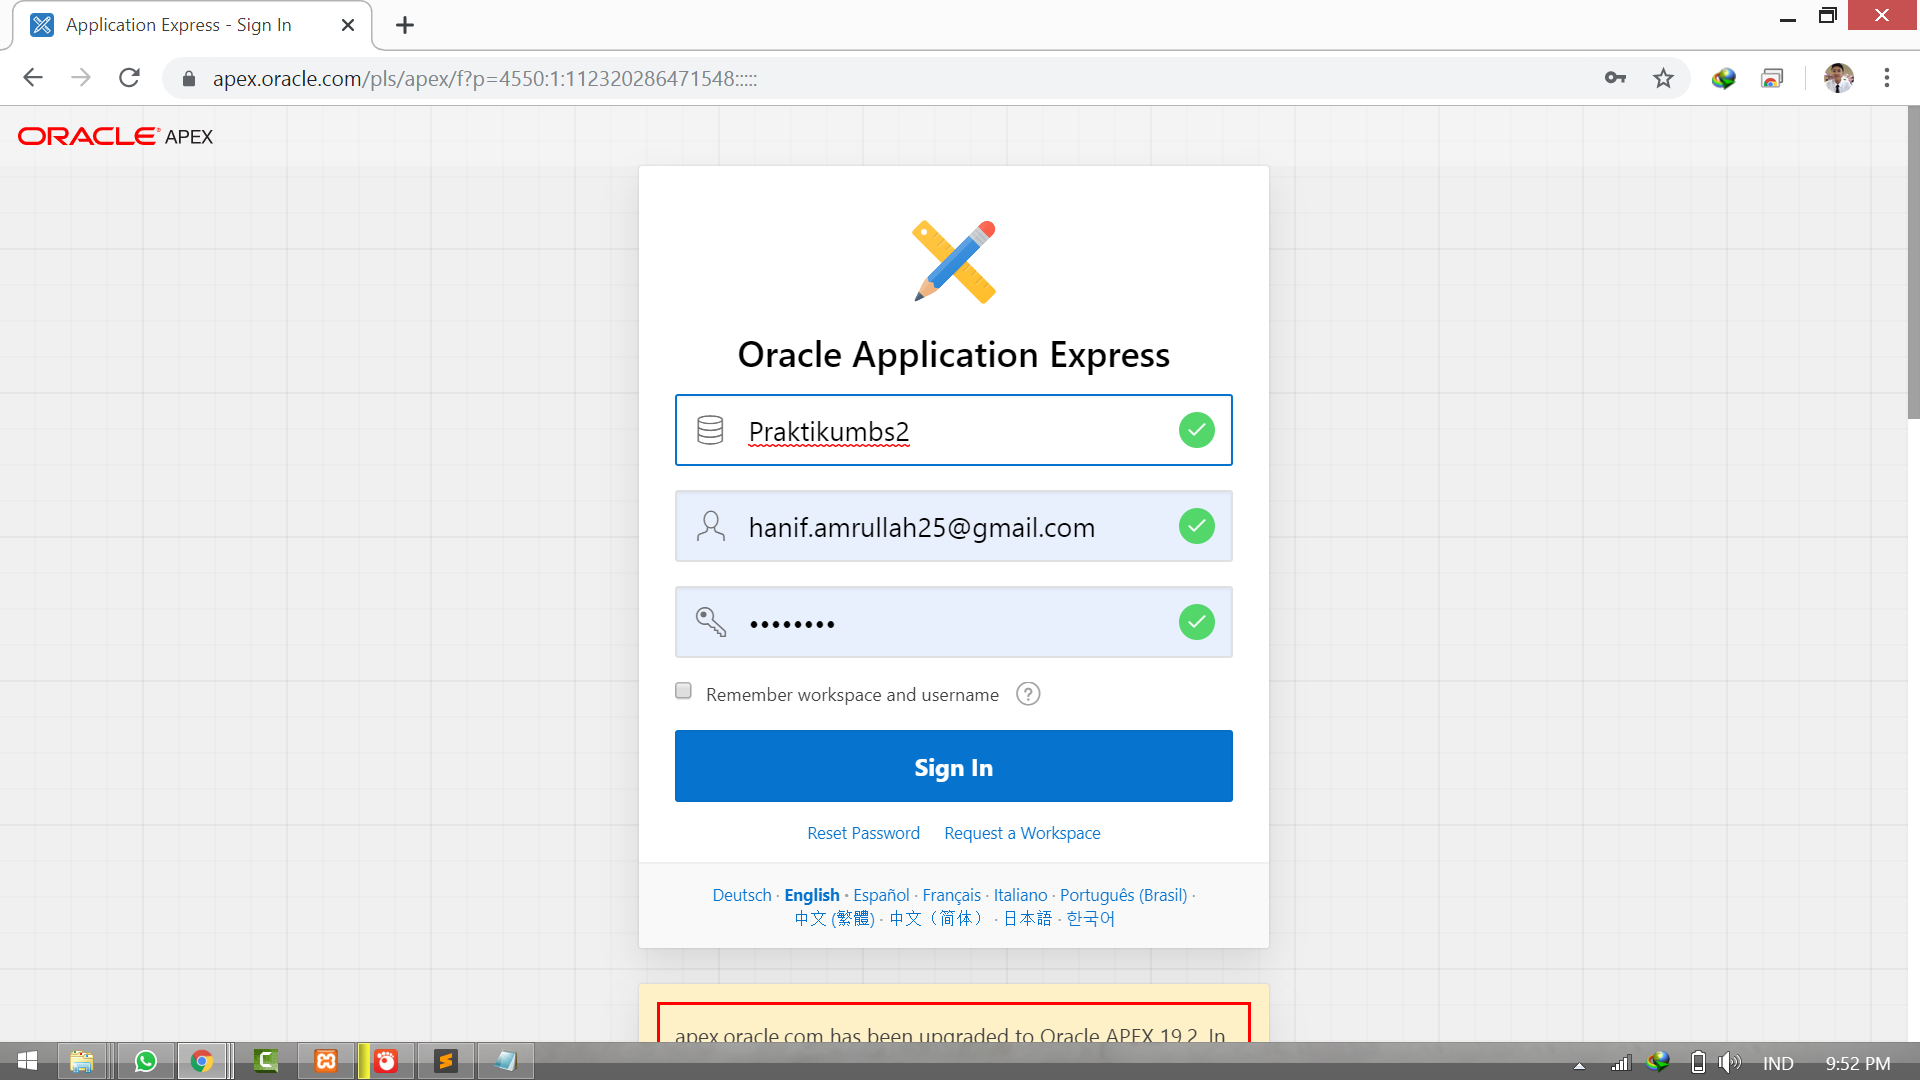
\includegraphics[width=8cm]{figure/1.png}}
            \end{figure}
            \item Pilih import atau pilih create jika belum mempunyai data
\begin{figure}[h]
\centerline{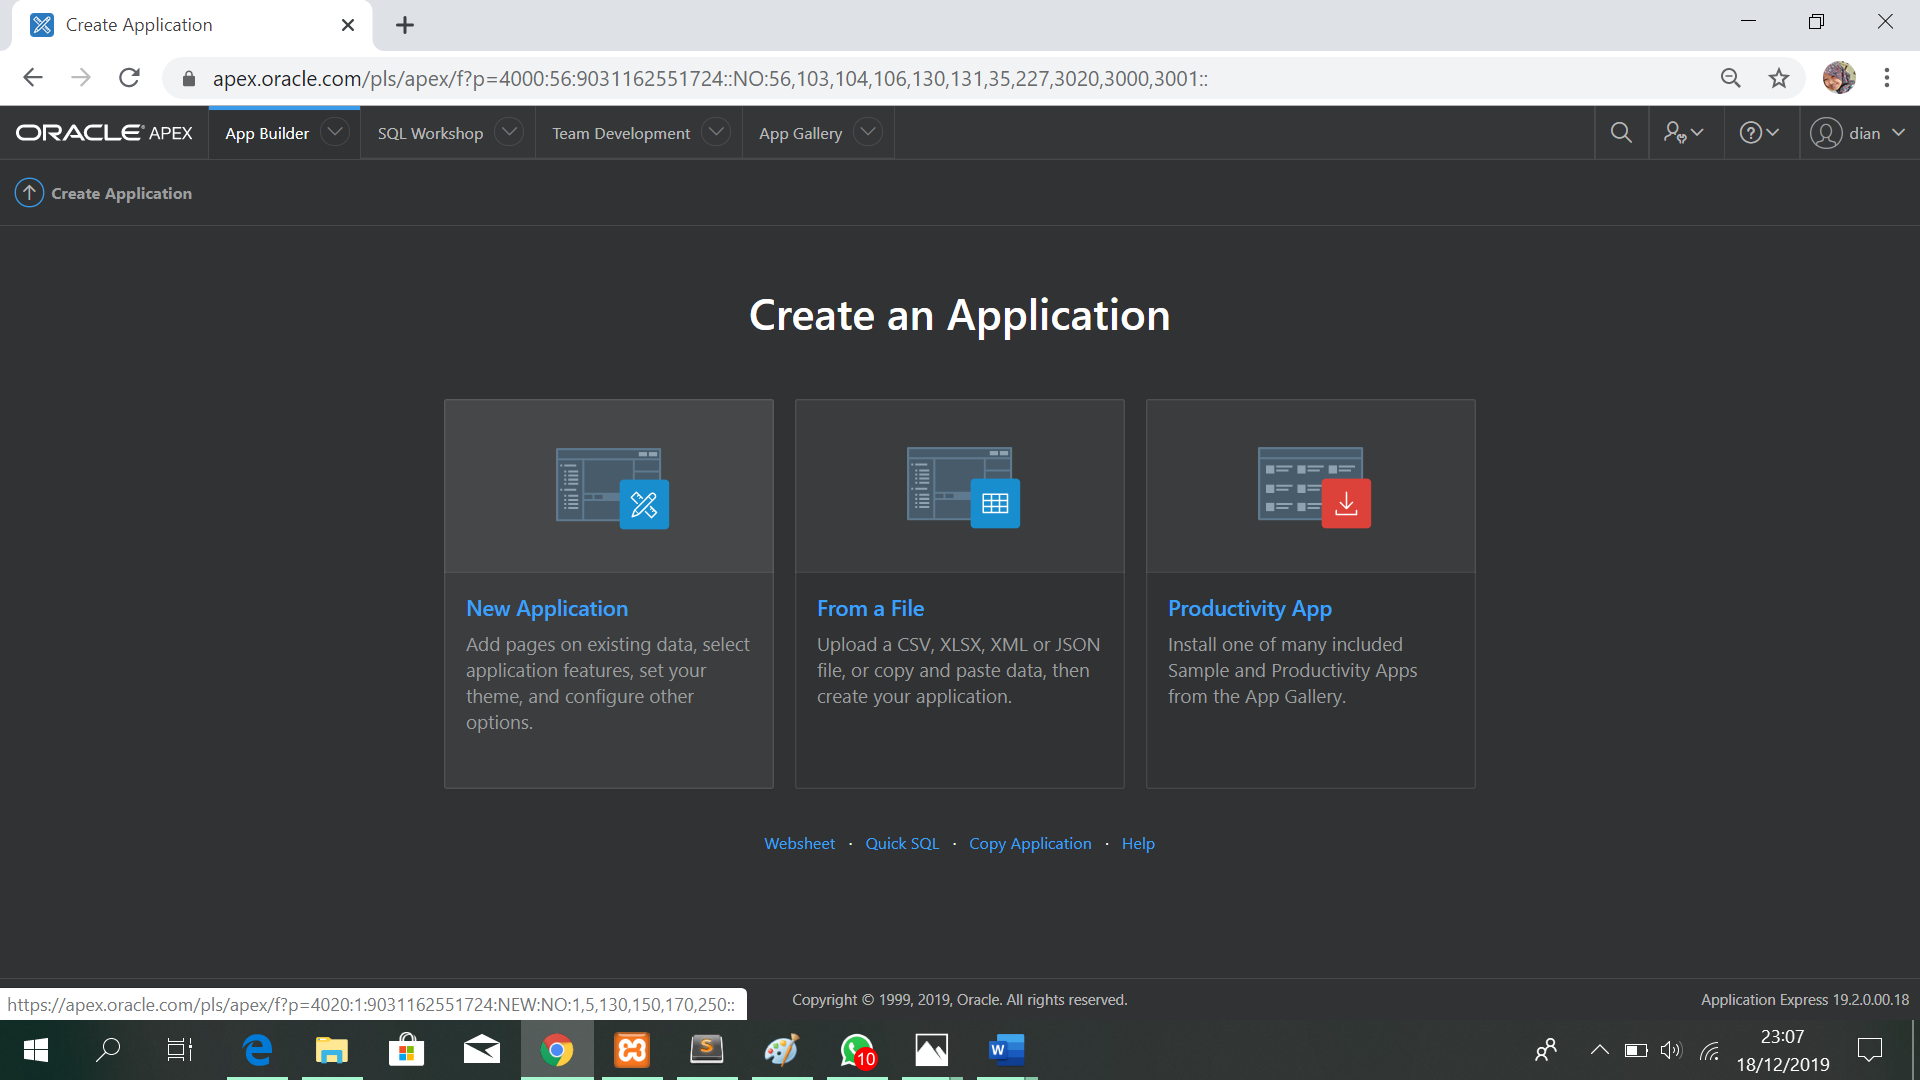
\includegraphics[width=8cm]{figure/2.png}}
            \end{figure}
         \item Pilih choose file lalu next.
\begin{figure}[h]
\centerline{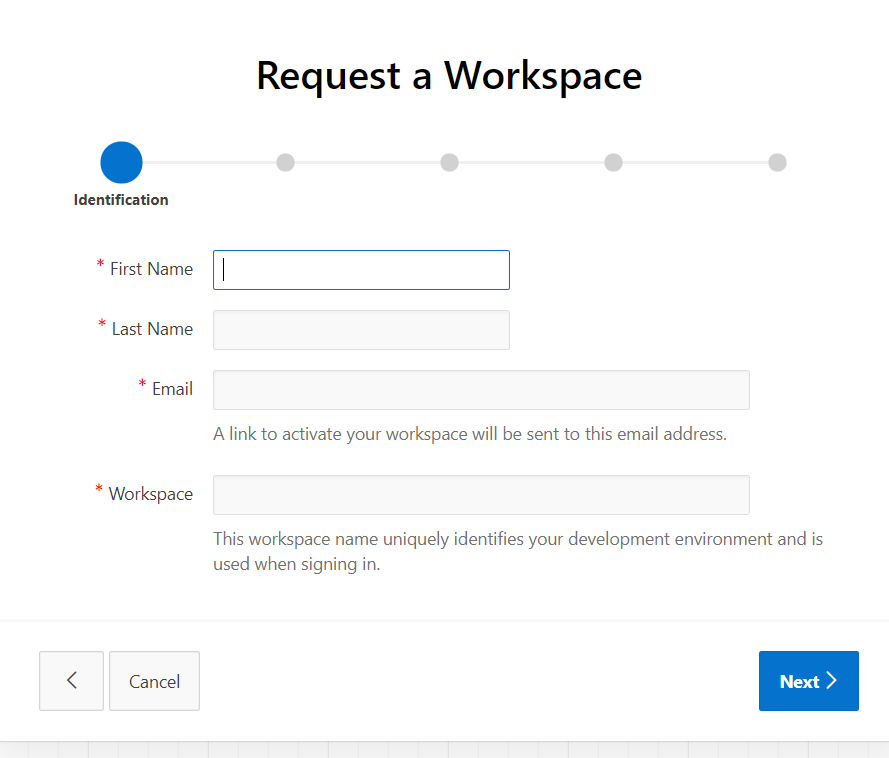
\includegraphics[width=8cm]{figure/3.png}}
            \end{figure}  
        \newpage \item Pilih next
\begin{figure}[h]
\centerline{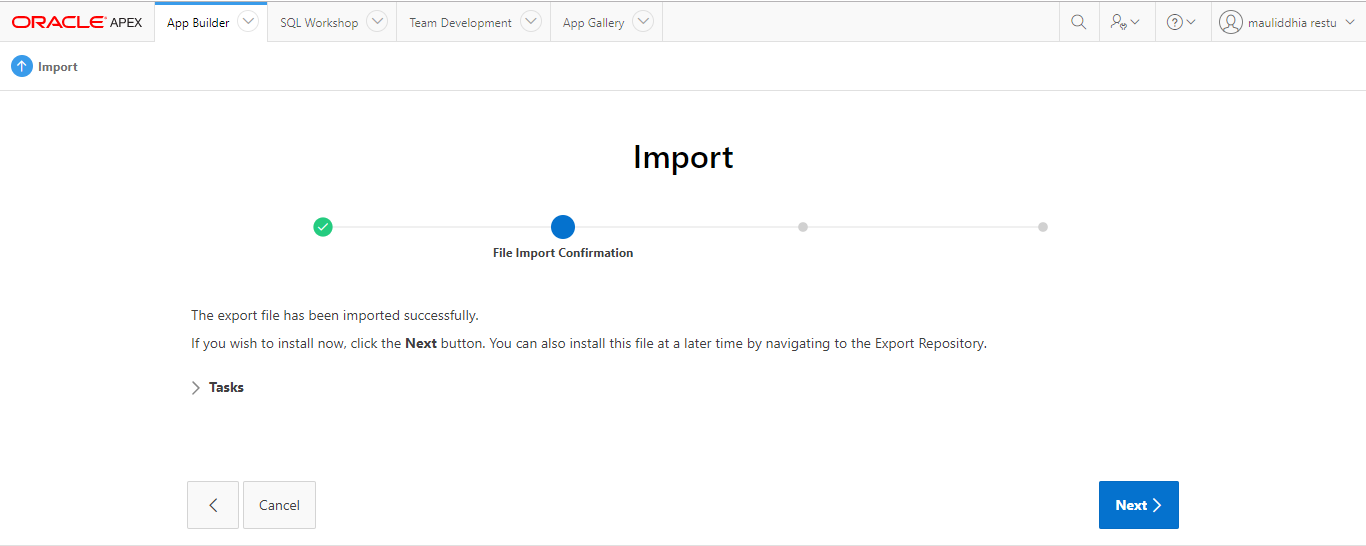
\includegraphics[width=8cm]{figure/4.png}}
            \end{figure}  
            \begin{figure}[h]
\centerline{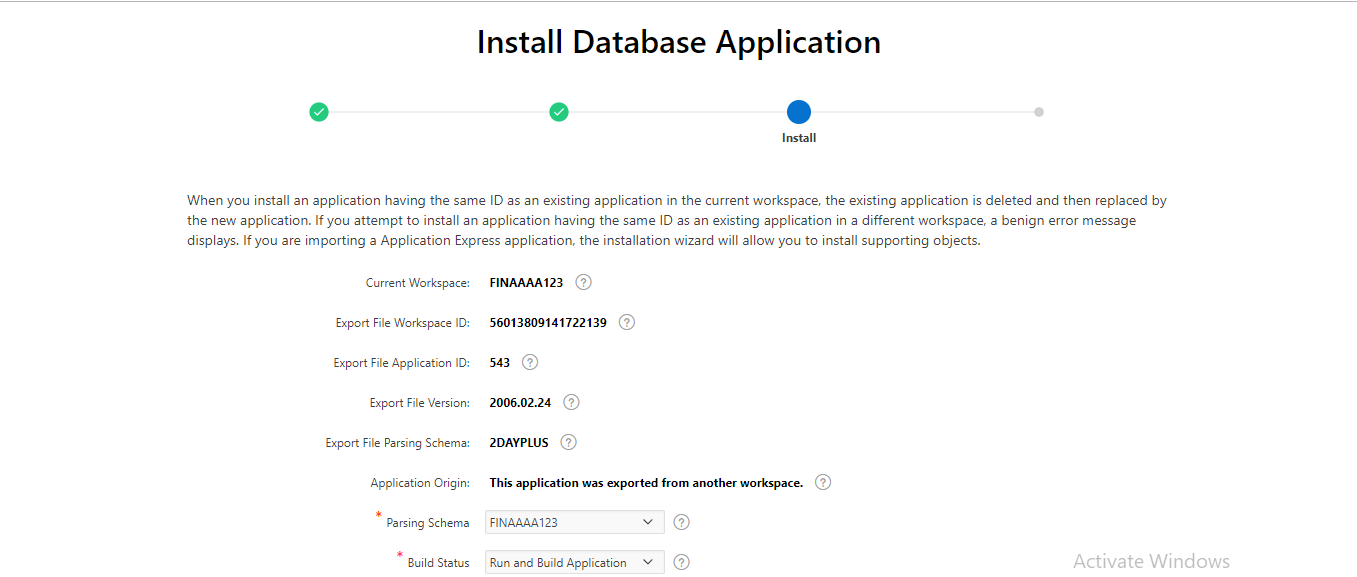
\includegraphics[width=8cm]{figure/5.png}}
            \end{figure}  
            \item lalu klik install application
\begin{figure}[h]
\centerline{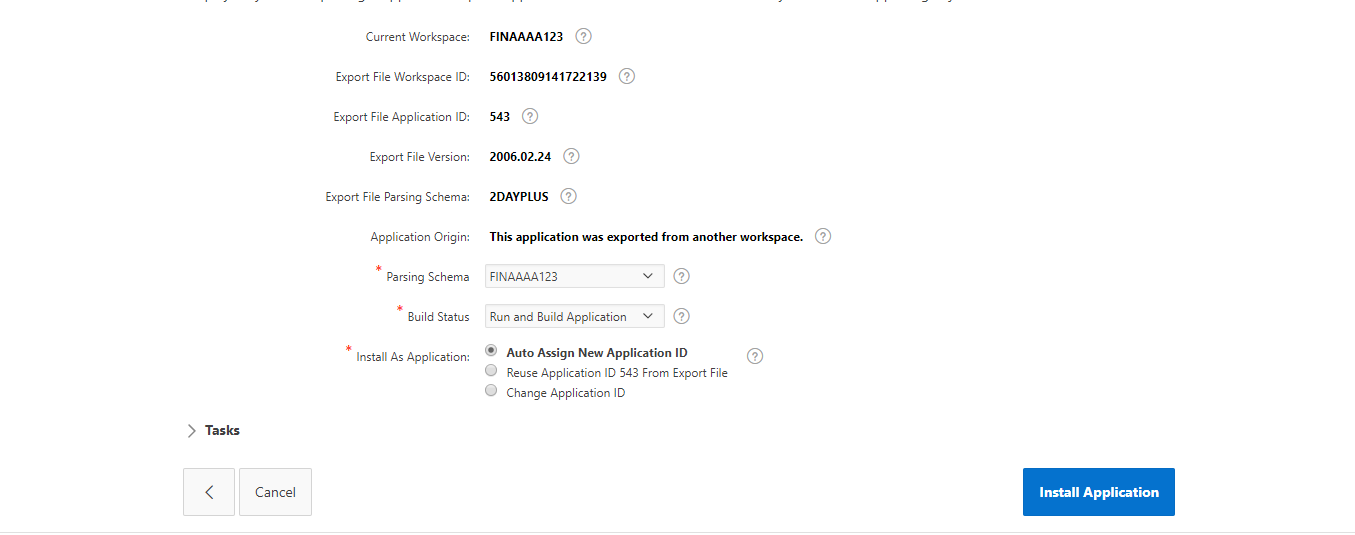
\includegraphics[width=8cm]{figure/6.png}}
            \end{figure}
           \newpage \item Pilih sql workshop,lalu pilih kembali objec browser untuk melihat apakah aplikasi yang di install tadi sudah terinstall atau belum
\begin{figure}[h]
\centerline{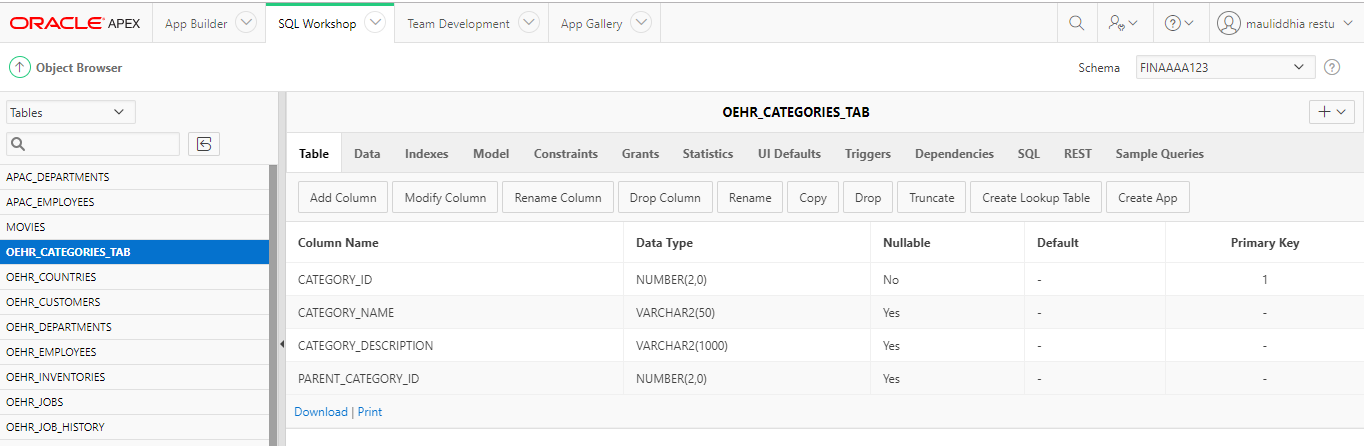
\includegraphics[width=8cm]{figure/7.png}}
            \end{figure}
            \item lalu kembali ke menu awal ,pilih app builder dan pilih create
\begin{figure}[h]
\centerline{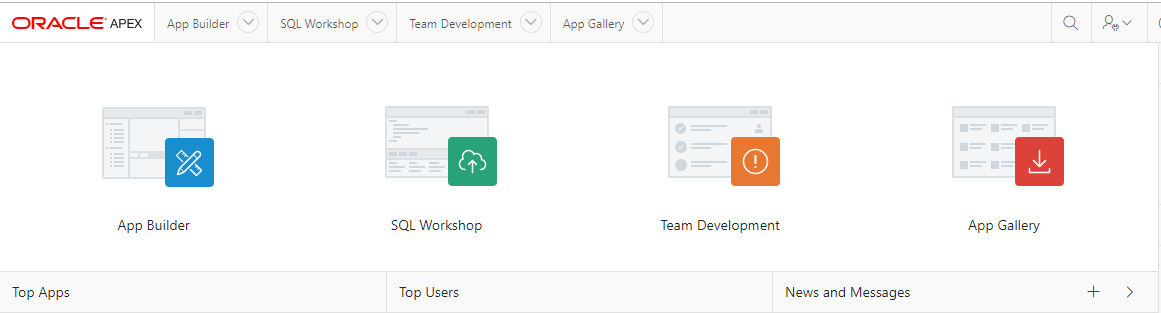
\includegraphics[width=8cm]{figure/8.png}}
            \end{figure}
            \newpage\item setelah itu pilih form a file
\begin{figure}[h]
\centerline{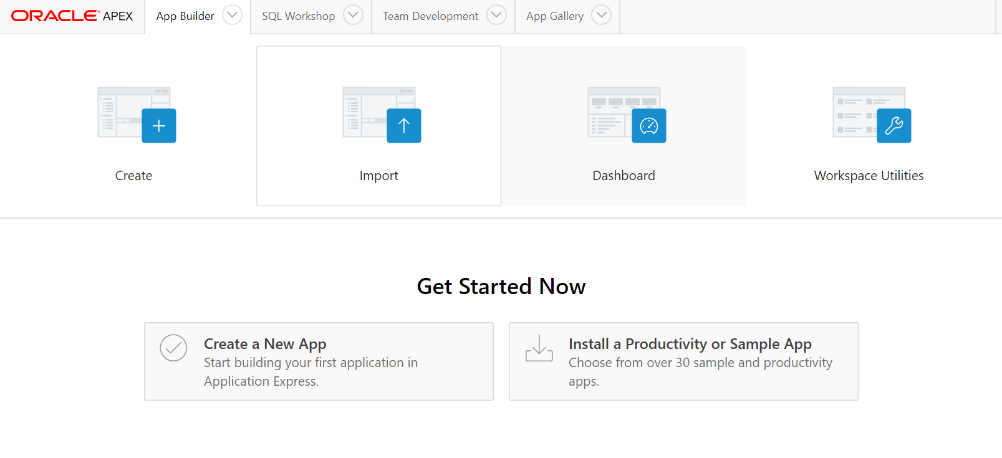
\includegraphics[width=8cm]{figure/9.png}}
            \end{figure}
            \item lalu pilih copy dan paste contoh file
\begin{figure}[h]
\centerline{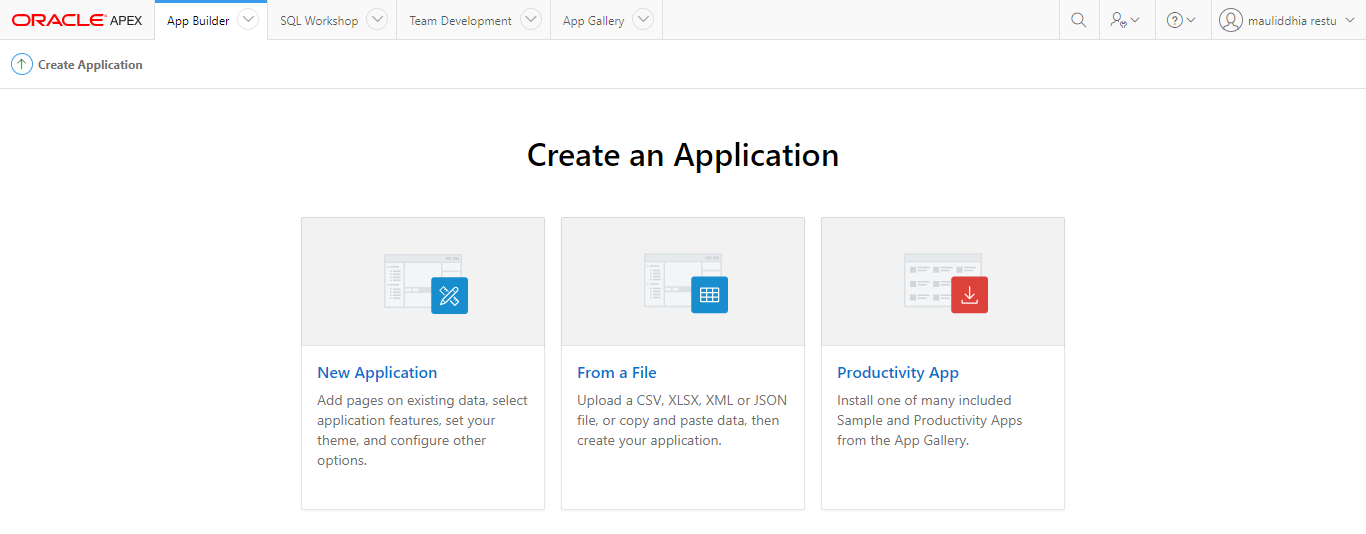
\includegraphics[width=8cm]{figure/10.png}}
            \end{figure}
            \item setelah itu  akan ada tampilan file yang telah dimasukkan dan pilih next
\begin{figure}[h]
\centerline{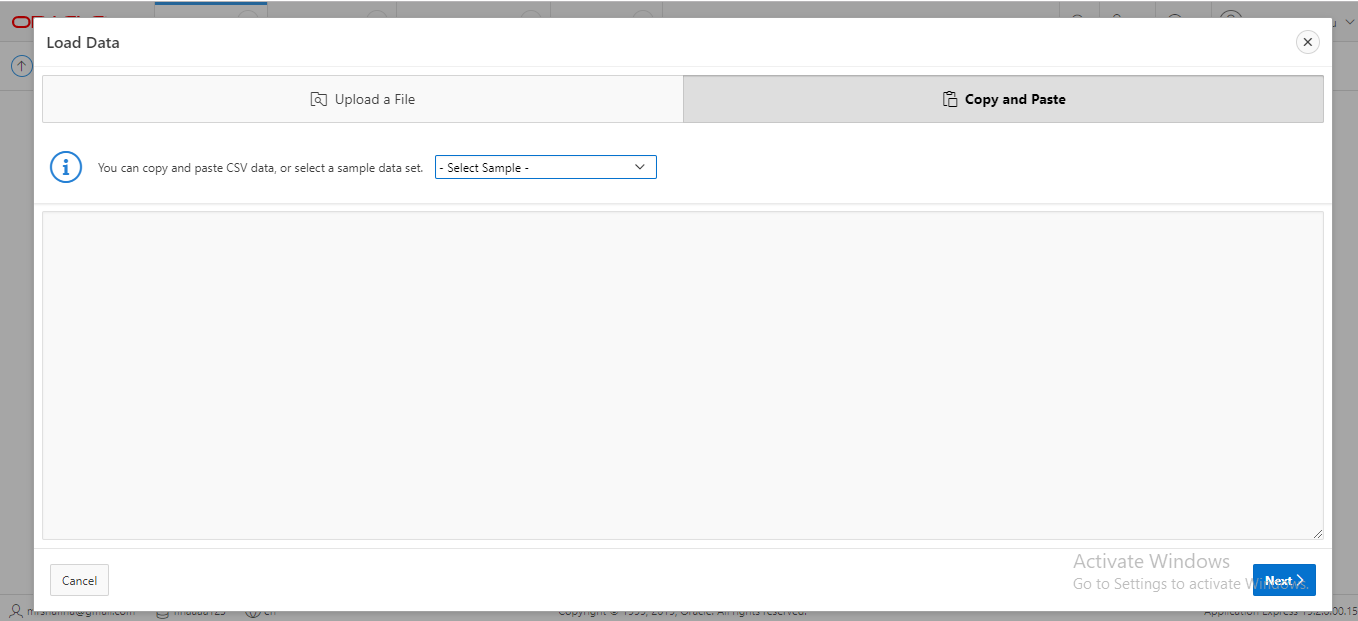
\includegraphics[width=8cm]{figure/11.png}}
            \end{figure}
           \newpage \item lalu isi nama table dan klik load data
\begin{figure}[h]
\centerline{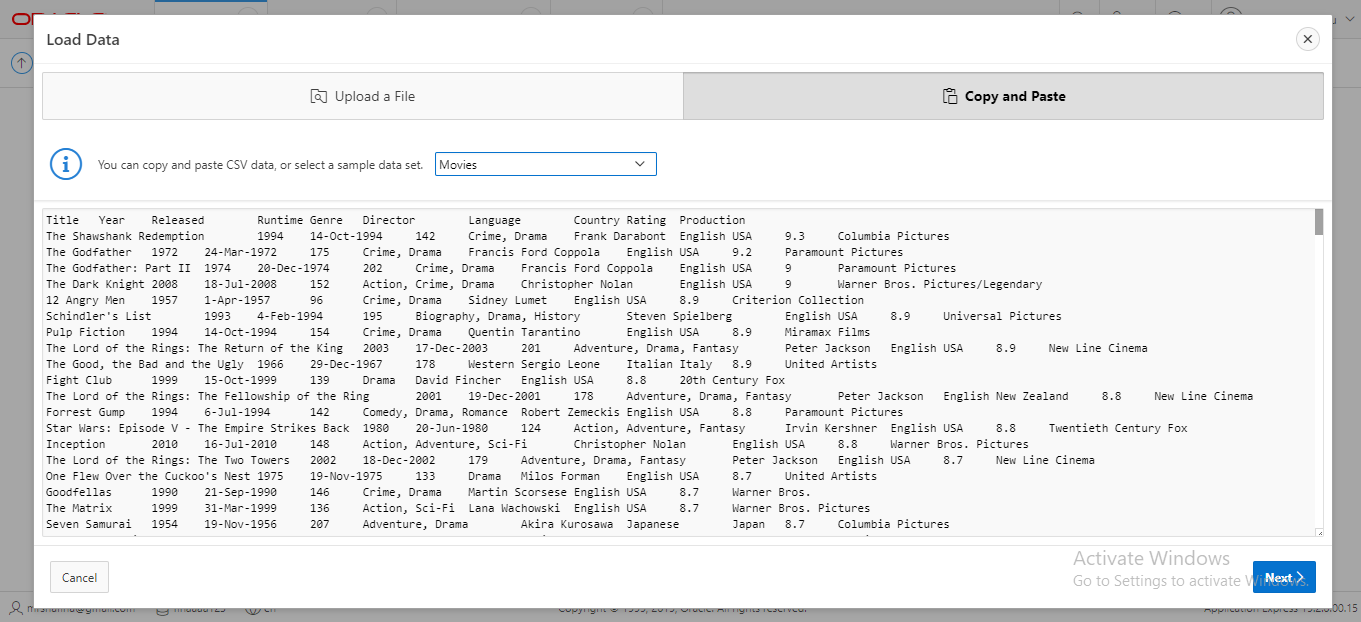
\includegraphics[width=8cm]{figure/12.png}}
            \end{figure}
            \item lalu tunggu sampai selesai
\begin{figure}[h]
\centerline{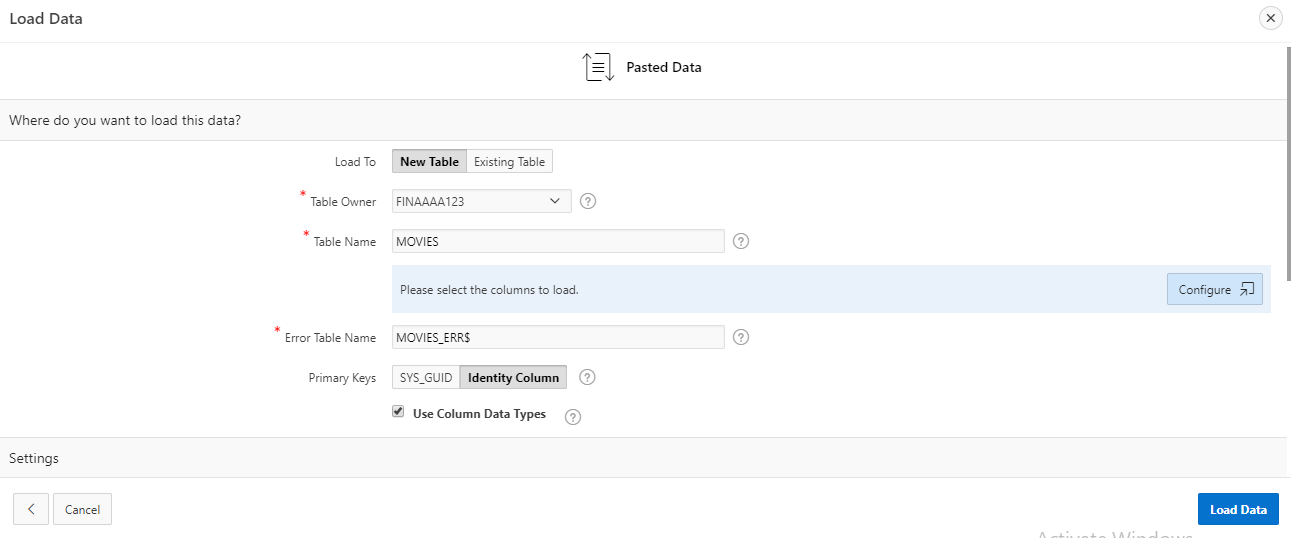
\includegraphics[width=8cm]{figure/13.png}}
            \end{figure}
            \item lalu akan ada tampilan seperti di bawah ini,lalu atur nama,page dan lain-lain
\begin{figure}[h]
\centerline{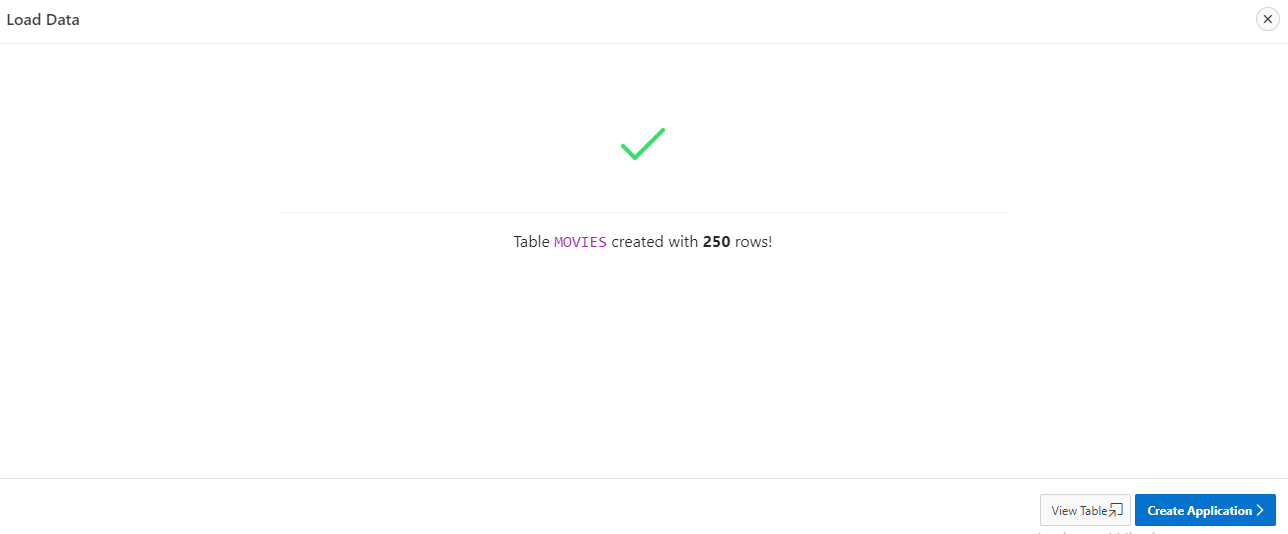
\includegraphics[width=8cm]{figure/14.png}}
            \end{figure}
           \newpage \item Pilih page yang diinginkan
\begin{figure}[h]
\centerline{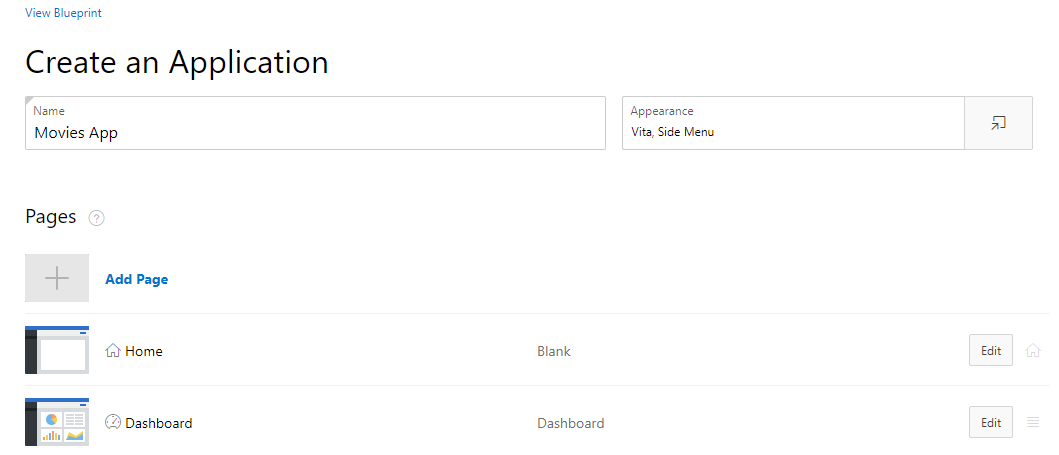
\includegraphics[width=8cm]{figure/15.png}}
            \end{figure}
            \item pada features jangan lupa check all,dan create application
\begin{figure}[h]
\centerline{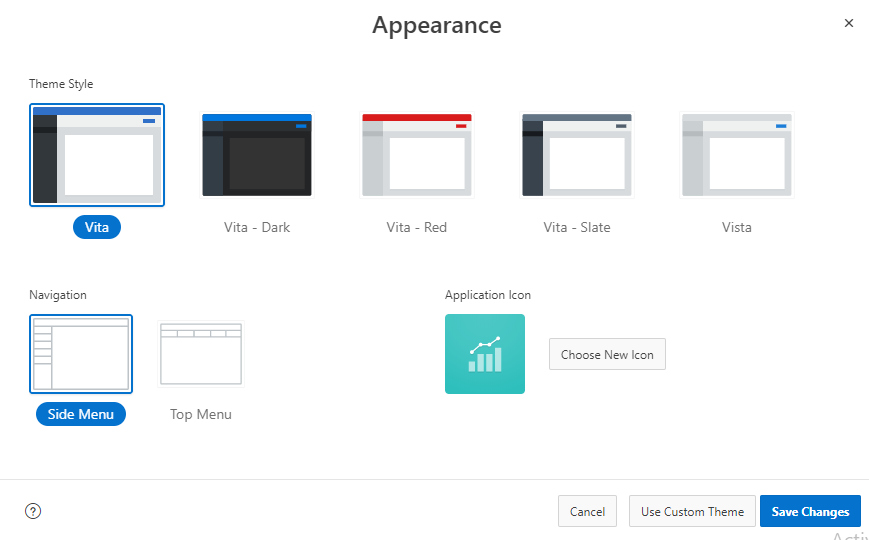
\includegraphics[width=8cm]{figure/16.png}}
            \end{figure}
            \item lalu run application
\begin{figure}[h]
\centerline{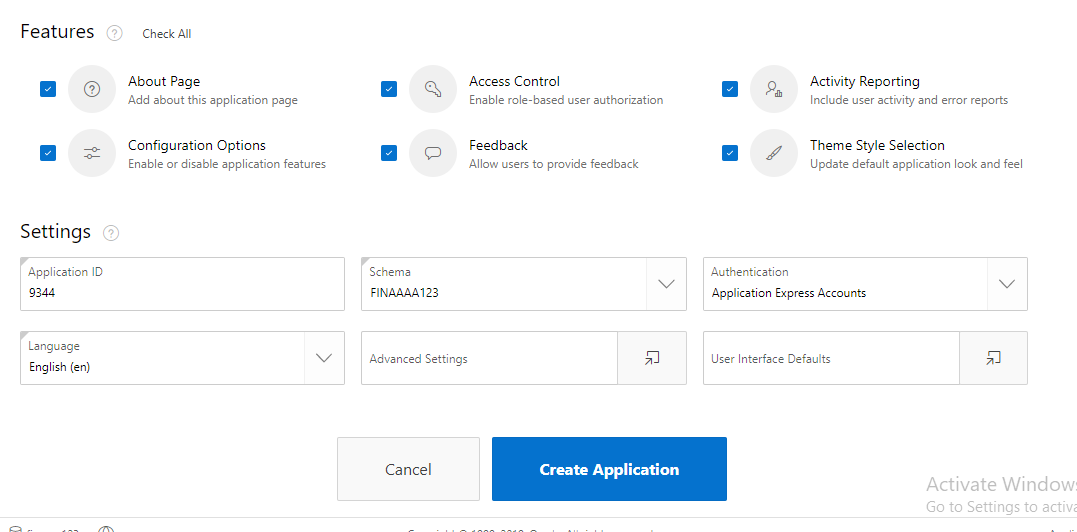
\includegraphics[width=8cm]{figure/17.png}}
            \end{figure}
           \newpage \item lalu masukkan username dan password
\begin{figure}[h]
\centerline{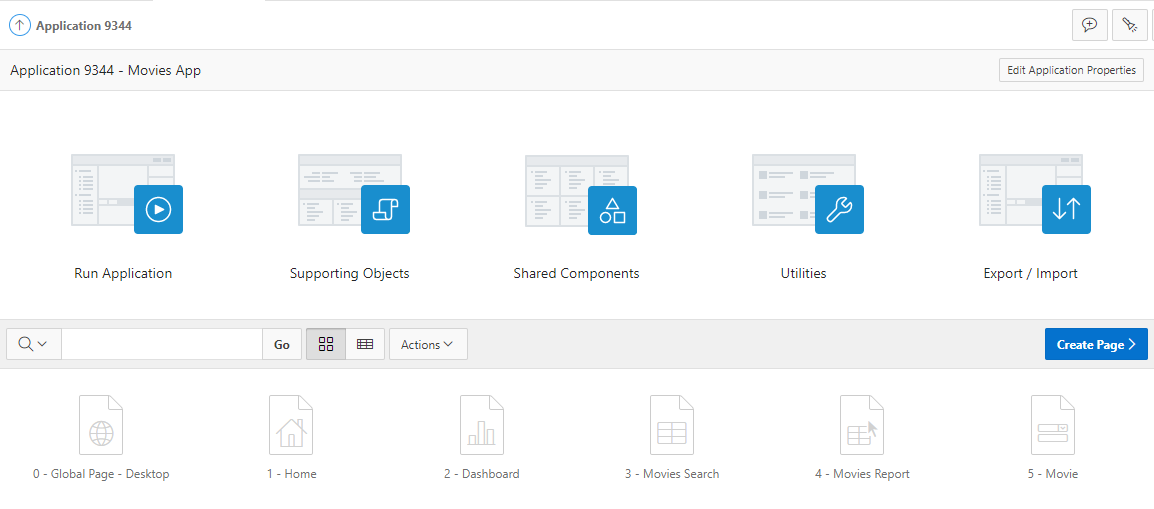
\includegraphics[width=8cm]{figure/18.png}}
            \end{figure}
            \item lalu akan masuk ke page atau aplikasi yang kalian buat
\begin{figure}[h]
\centerline{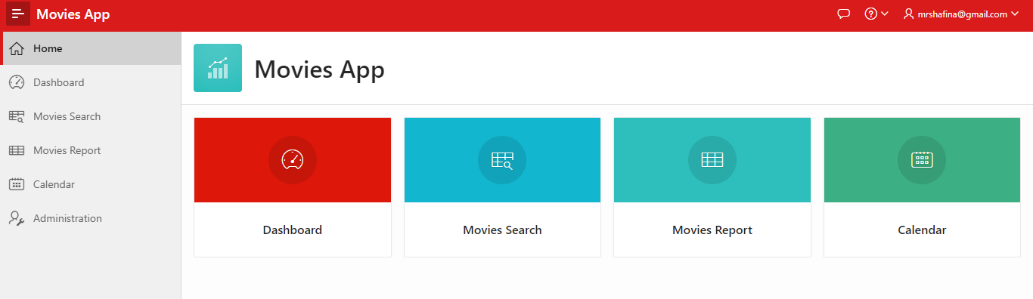
\includegraphics[width=8cm]{figure/20.png}}
            \end{figure}
            
\end{enumerate}
\section{Quick SQL}
\begin{enumerate}
\item Masuk Ke Oracle, pilih sign in
\begin{figure}[h]
\centerline{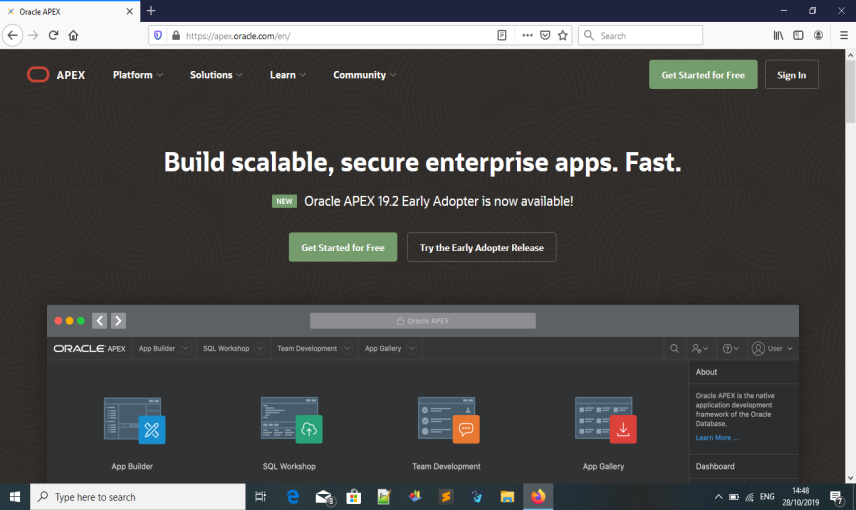
\includegraphics[width=8cm]{figure/si.png}}
\end{figure}
 \item Lalu masukkan workspacae,username,dan password yang kalian punya atau buat aku jika kalian belum mempunyai akun.
\begin{figure}[h]
\centerline{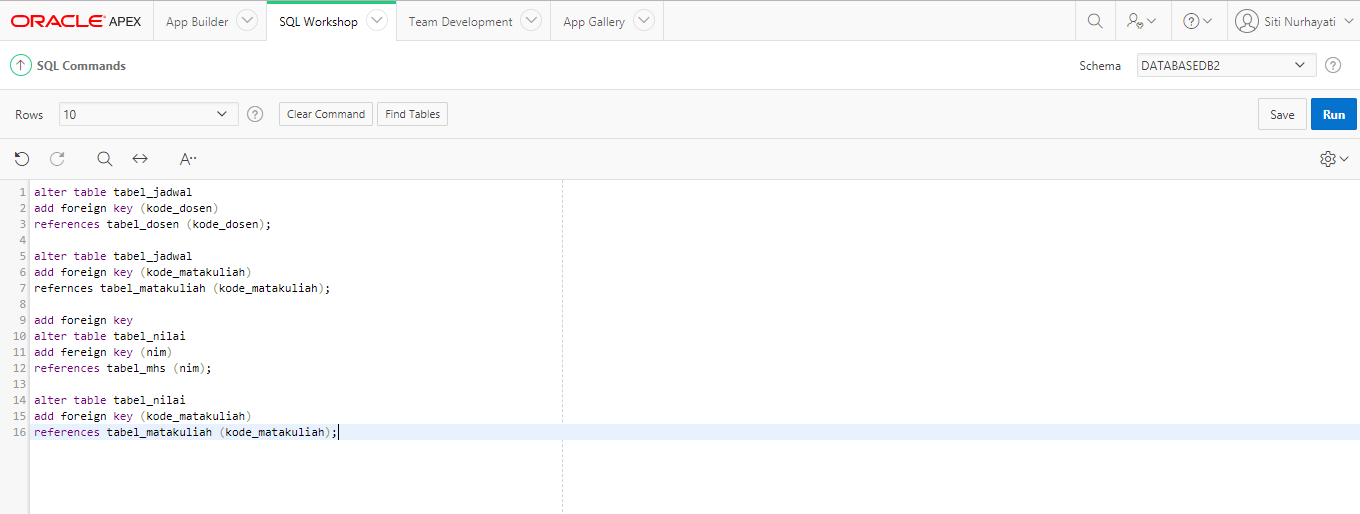
\includegraphics[width=8cm]{figure/a.png}}
\end{figure}
 \newpage\item Setelah itu akan muncul tampilan seperti dibawah ini. Lalu pilih sql workshop dan pilih utilities kemudia pilih quick sql.
\begin{figure}[h]
\centerline{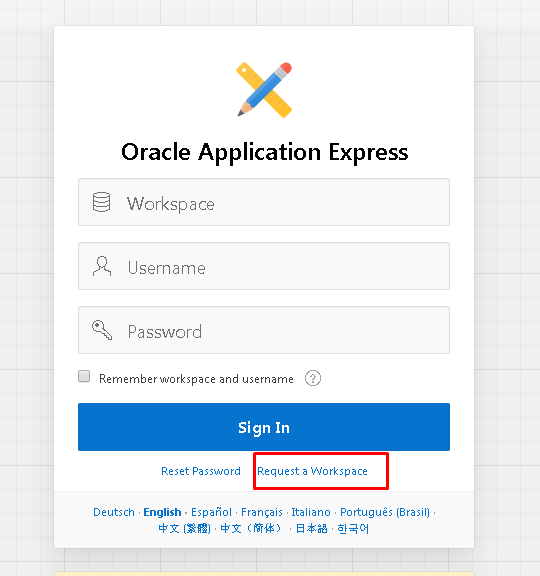
\includegraphics[width=8cm]{figure/b.png}}
\end{figure}
\item lalu akan muncul tampilan seperti ini.  Maka setelah itu kalian dapat menuliskan kodingan atau program yang akan di jalankan .
\begin{figure}[h]
\centerline{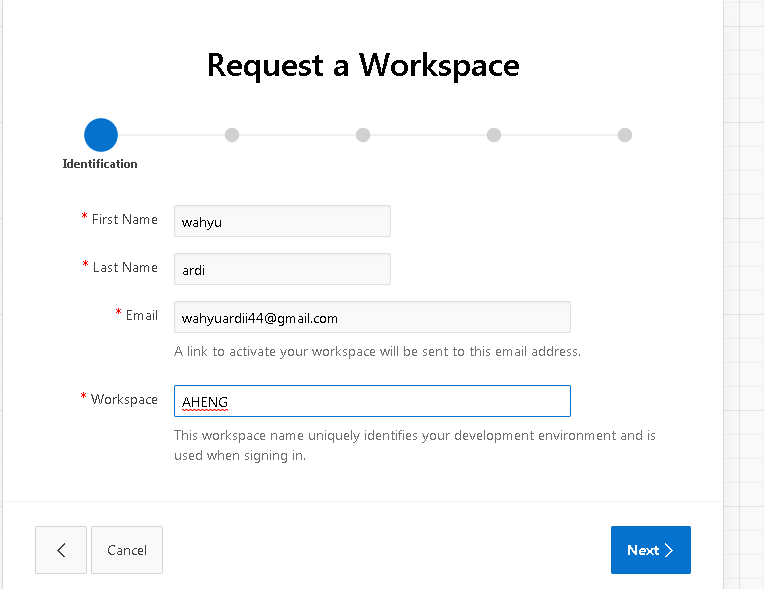
\includegraphics[width=8cm]{figure/c.png}}
\end{figure}
\newpage\item Setelah itu pilih sql workshop.  
\begin{figure}[h]
\centerline{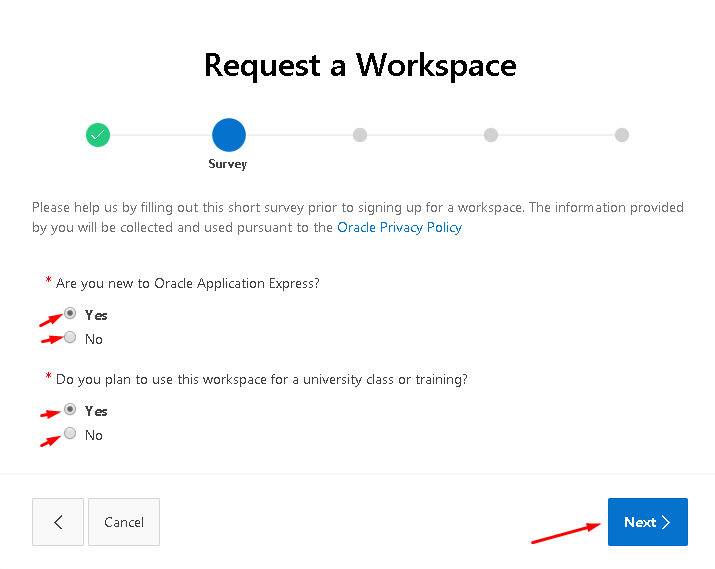
\includegraphics[width=8cm]{figure/d.png}}
            \end{figure}
\item Setelah itu pilih sql scripts.  
               \begin{figure}[h]
\centerline{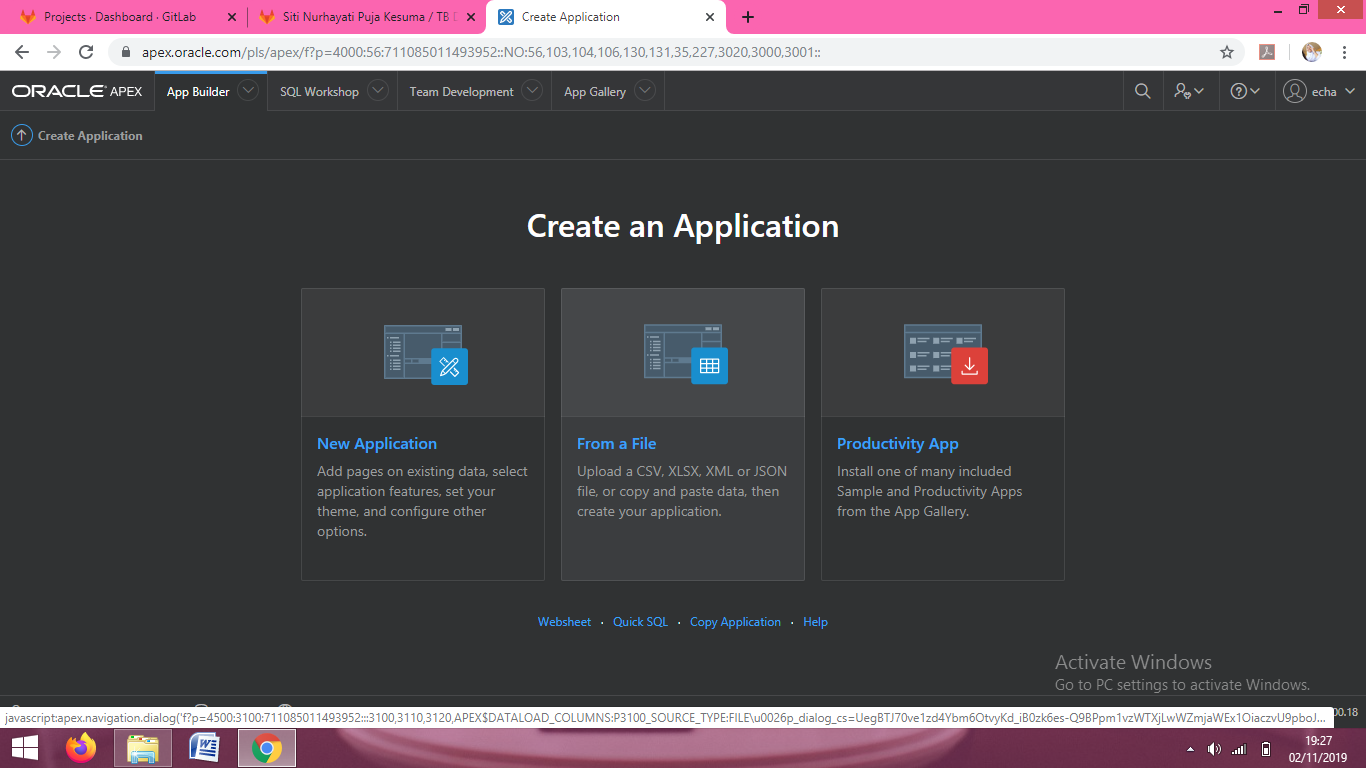
\includegraphics[width=8cm]{figure/e.png}}
            \end{figure}
\newpage \item  maka kalian akan melihat seperti ini lalu pindahkan kodingan atau program yang kita tulis di quick sql.  
               \begin{figure}[h]
\centerline{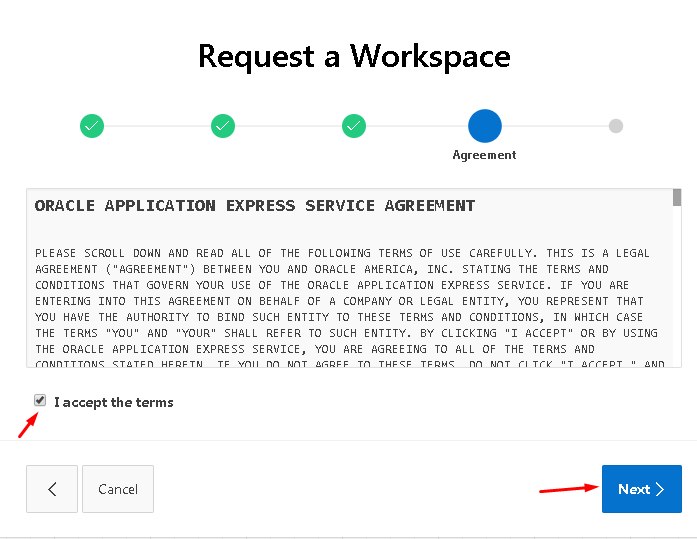
\includegraphics[width=8cm]{figure/f.png}}
            \end{figure}
\item  setelah itu run script
               \begin{figure}[h]
\centerline{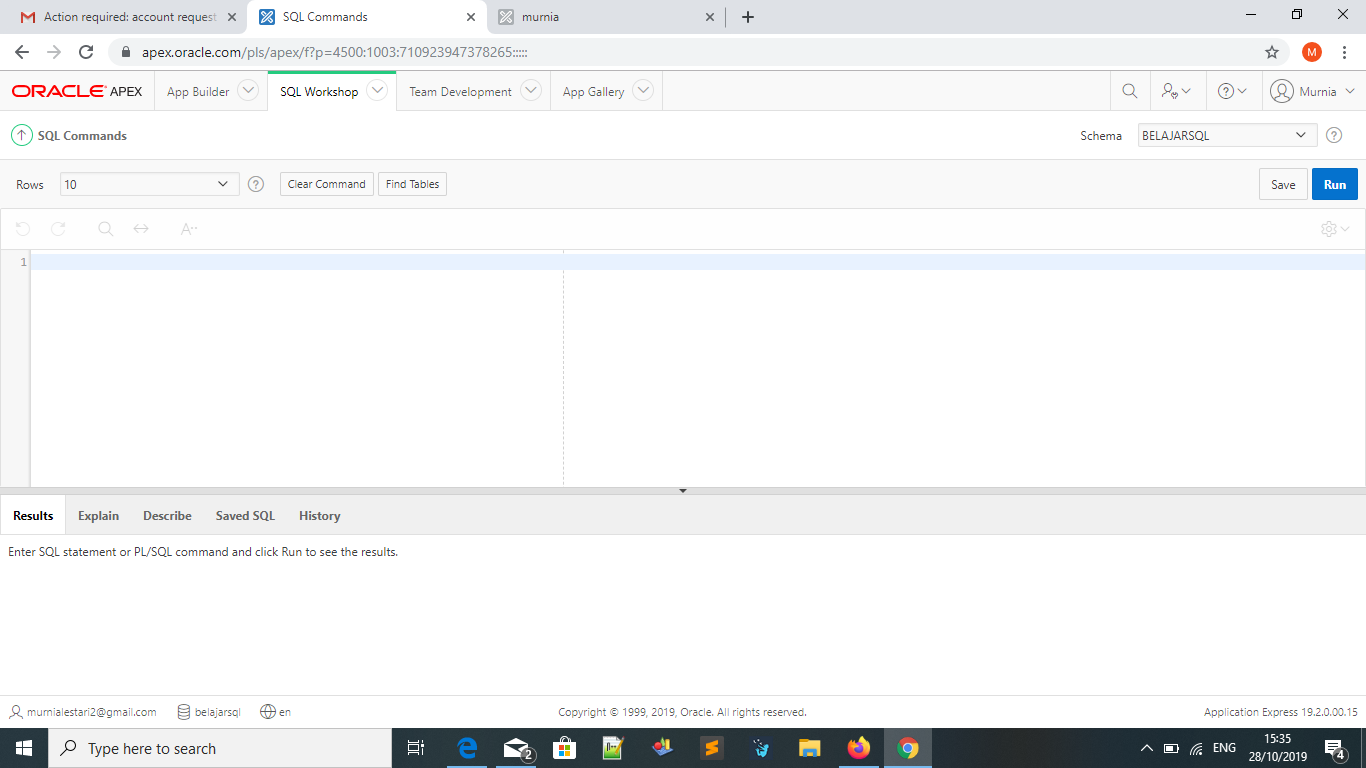
\includegraphics[width=8cm]{figure/g1.png}}
            \end{figure}     
\item  Setelah itu pilih sql command untuk memanggil kodingan atau program yang kita buat
               \begin{figure}[h]
\centerline{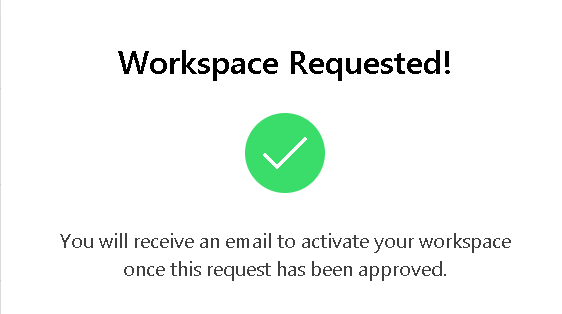
\includegraphics[width=8cm]{figure/h.png}}
            \end{figure}
            

    
\end{enumerate}
\section{Aplikasi development}
\begin{enumerate}

\item Buka ilearning.oracle

 
\item Lalu download modul yang kalian mau pada ilearning.
\begin{figure}[h]
\centerline{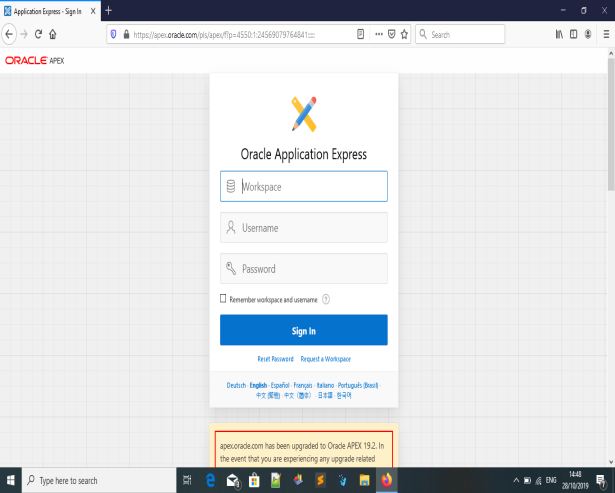
\includegraphics[width=8cm]{figure/B.png}}
            \end{figure}
\item Lalu masuk ke oracleapex.com

 
\newpage\item Lalu akan keluar tampilan awal pada oracle apex
\begin{figure}[h]
\centerline{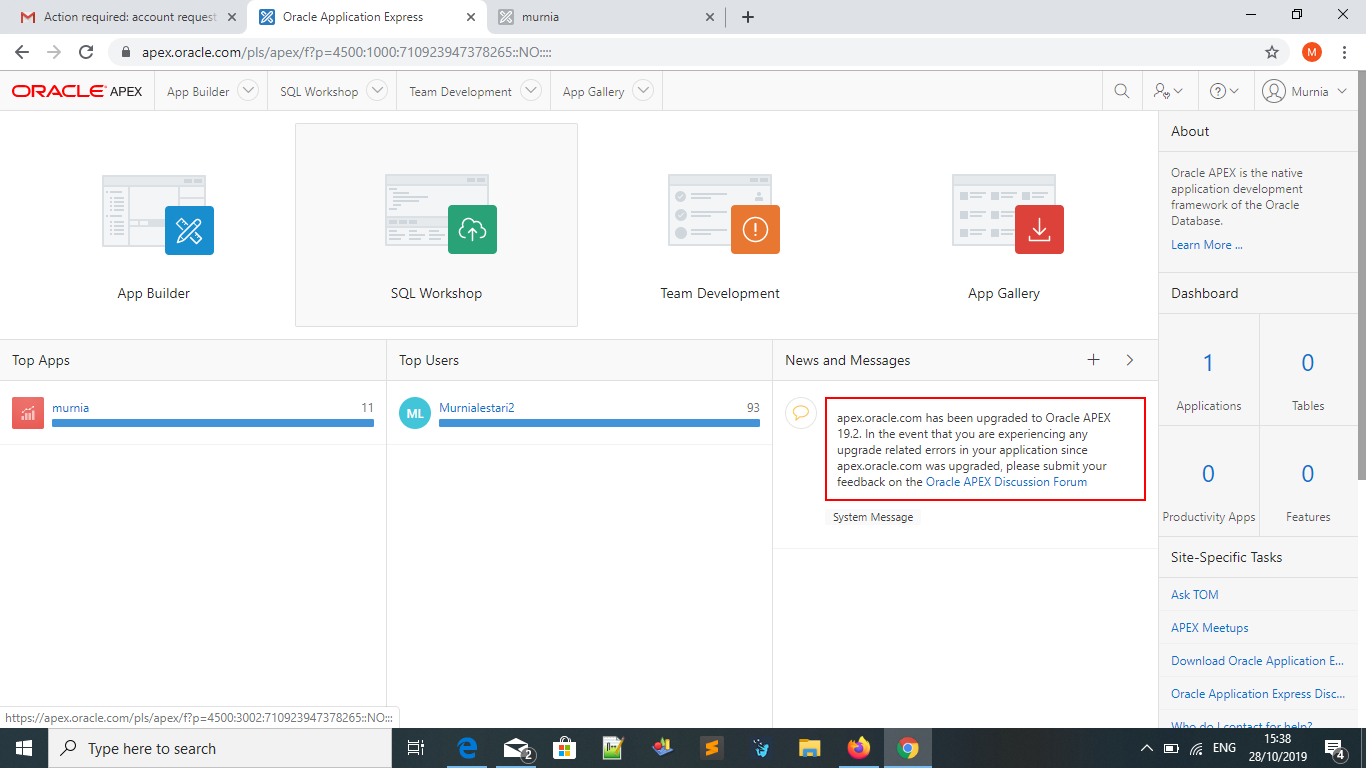
\includegraphics[width=8cm]{figure/C.png}}
            \end{figure}
 
\item  Kemudian pilih sql workshop
\begin{figure}[h]
\centerline{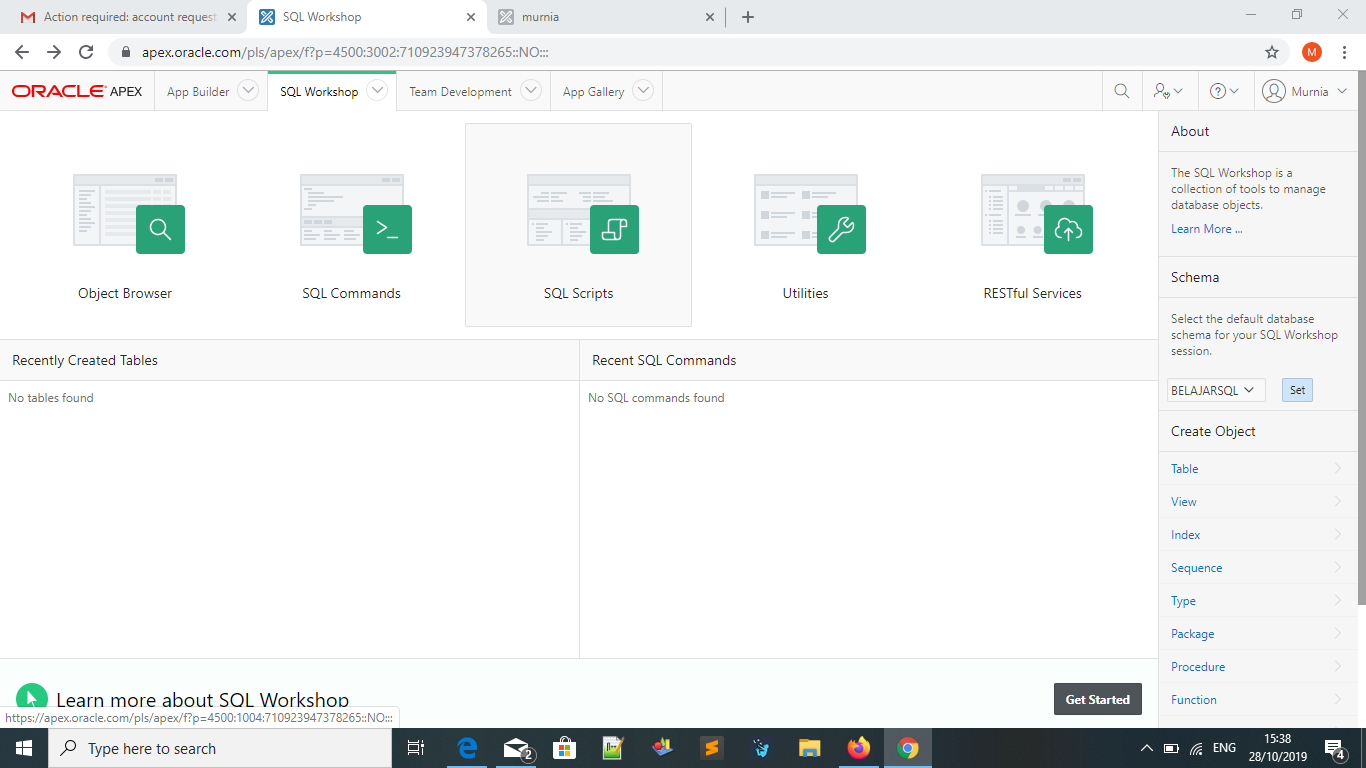
\includegraphics[width=8cm]{figure/D.png}}
            \end{figure}
 
\newpage\item  Lalu pilih sql script
\begin{figure}[h]
\centerline{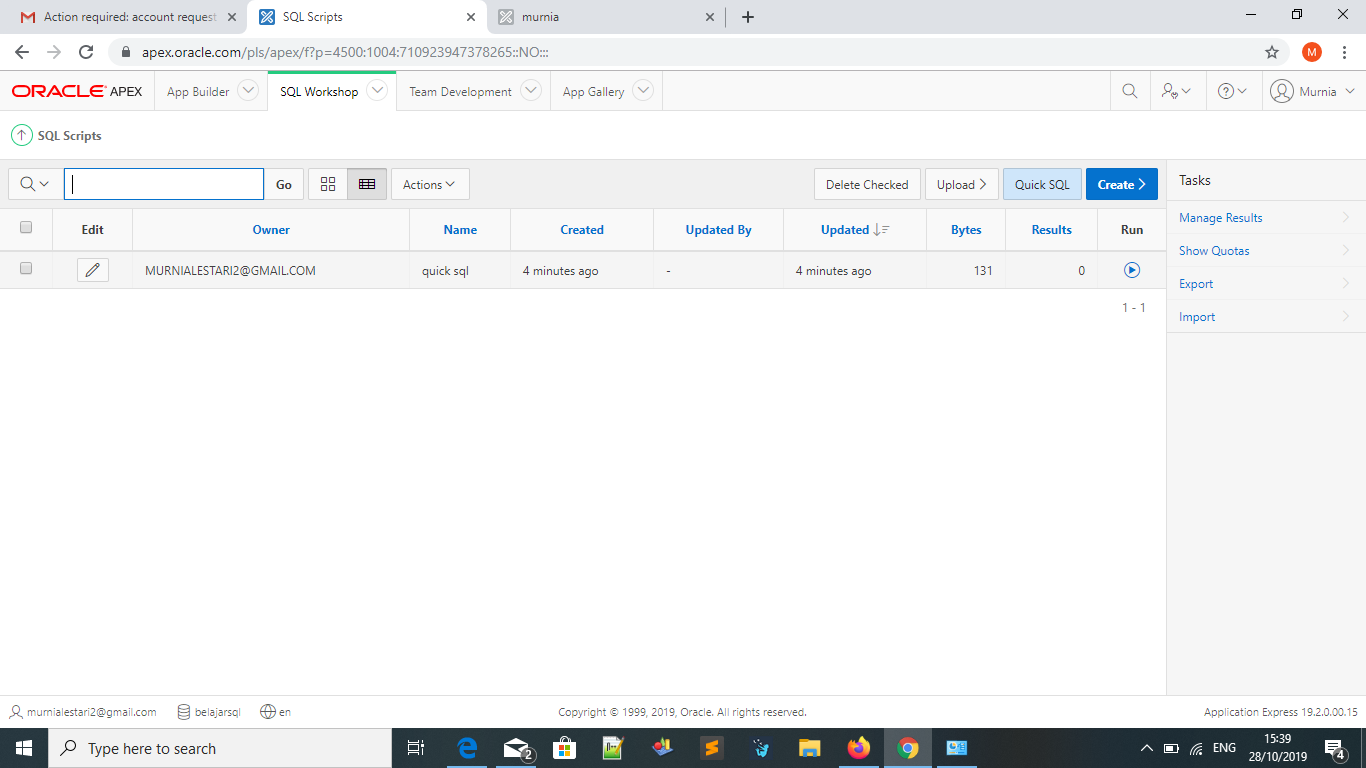
\includegraphics[width=8cm]{figure/E.png}}
            \end{figure}
 
\item  kemudian pilih upload script, maka pilih lah file yang akan dimasukkan ke dalam sql script . kemudian akan muncul file yang telah dimasukkan
\item  Lalu tekan tombol run
\item  Setelah itu pergi ke tampilan awal dan pilih aplikasi builder,lalu pilih desktop
\begin{figure}[h]
\centerline{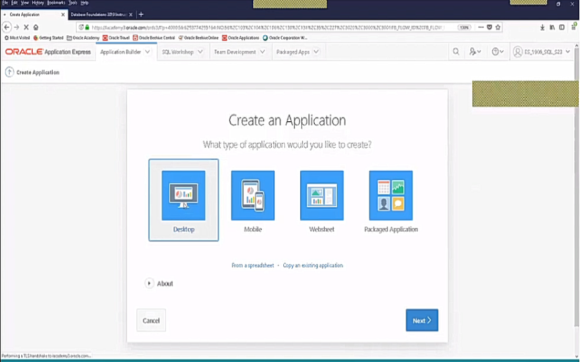
\includegraphics[width=8cm]{figure/F.png}}
            \end{figure}
 
\newpage\item  Lalu  Create Aplikasi baru , jangan lupa Menganti nama menjadi Employe Database Aplication , kemudia Next
\begin{figure}[h]
\centerline{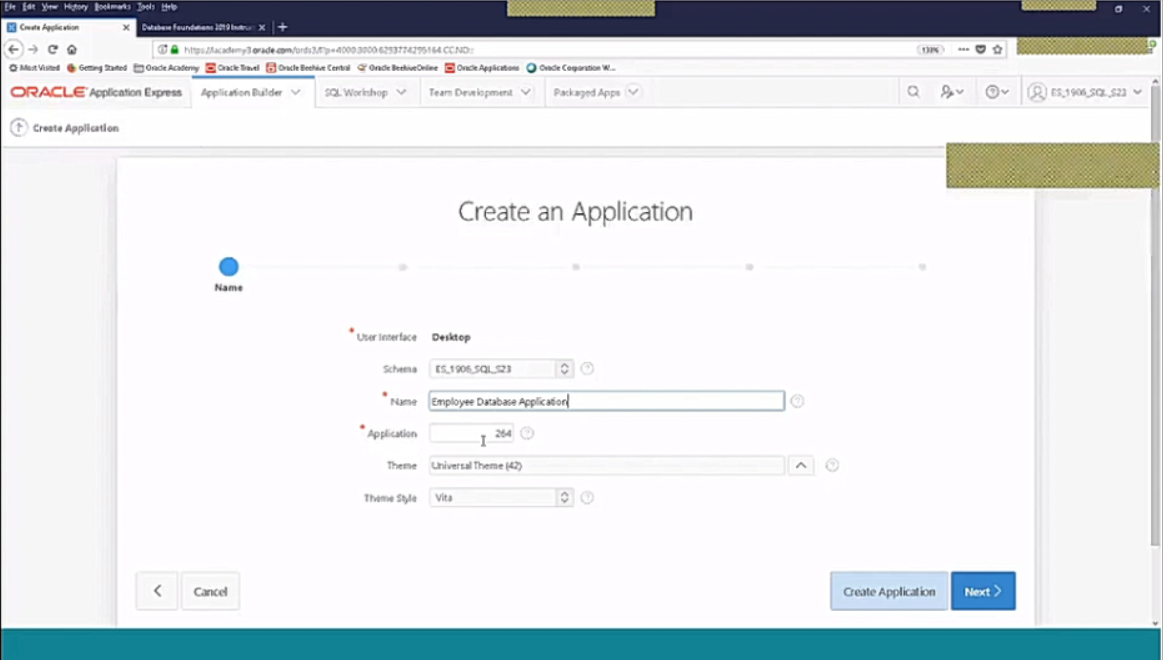
\includegraphics[width=8cm]{figure/G.png}}
            \end{figure}

\item  Lalu setelah halaman telah berpindah , akan tampak seperti dibawah ini, kemudian table akan muncul dan klik next. 
\begin{figure}[h]
\centerline{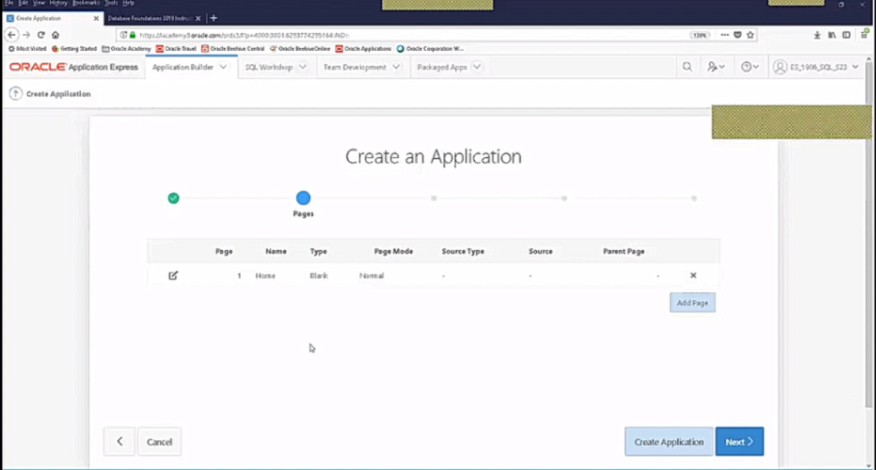
\includegraphics[width=8cm]{figure/H.png}}
            \end{figure}

\item  Setelah itu akan muncul seperti dibawah ini, dan pilih report dan add page kemudian  klik next.
\begin{figure}[h]
\centerline{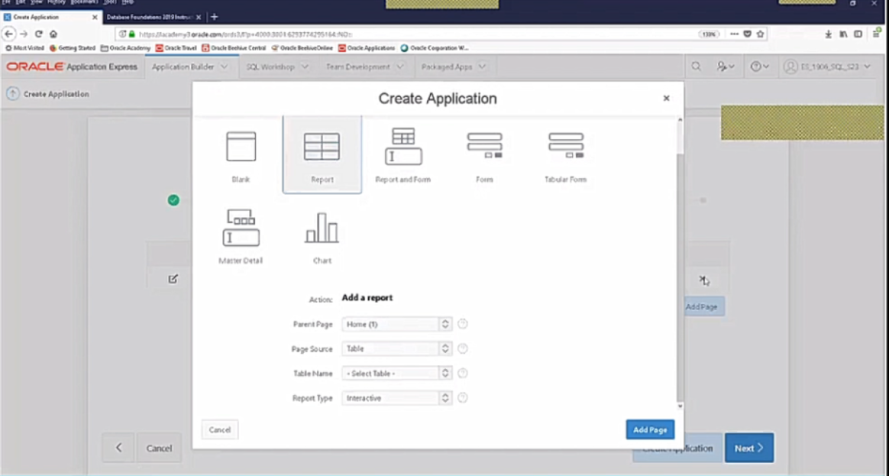
\includegraphics[width=8cm]{figure/I.png}}
            \end{figure}
\item  Lalu pilih NO dan klik Next
\begin{figure}[h]
\centerline{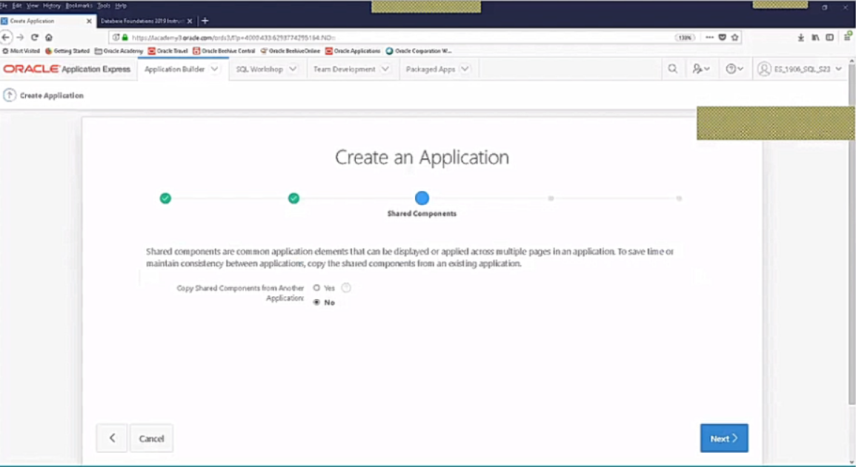
\includegraphics[width=8cm]{figure/J.png}}
            \end{figure}
\item  Lalu pada bagian ini ganti application schema menjadi No Autentication, kemudian next
\begin{figure}[h]
\centerline{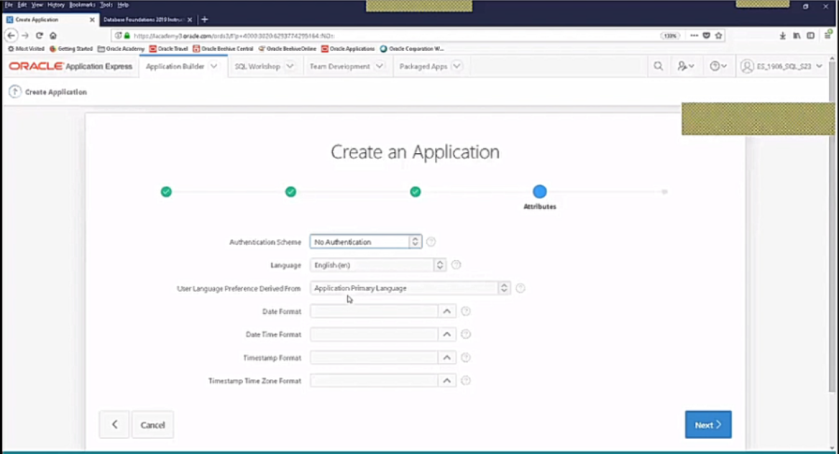
\includegraphics[width=8cm]{figure/K.png}}
            \end{figure}
\item  Karena  table sudah  dibuat, maka klik create application
\begin{figure}[h]
\centerline{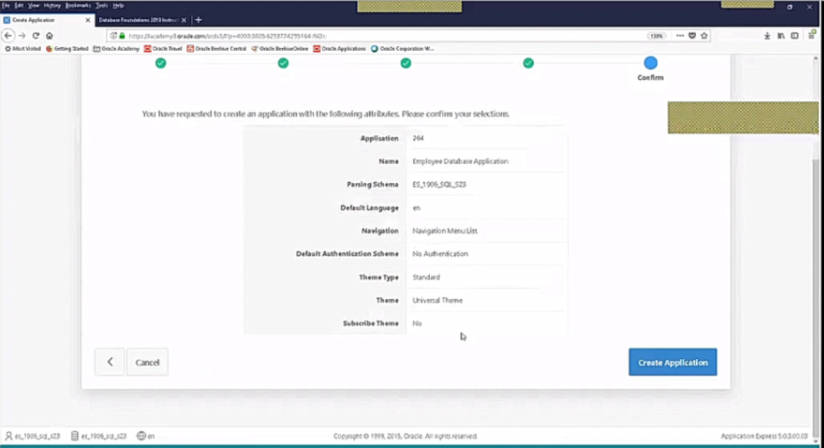
\includegraphics[width=8cm]{figure/L.png}}
            \end{figure}
\newpage\item   Lalu Akan muncul kalimat Aplication create successfully maka sudah berhasil membuat aplikasi table nya dulu.
jangan lupa untuk view Schema agar bisa liat apa yang telah kita buat.
\begin{figure}[h]
\centerline{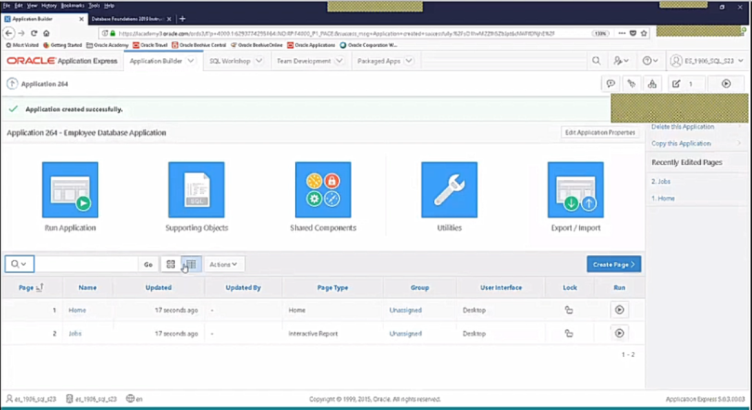
\includegraphics[width=8cm]{figure/M.png}}
            \end{figure}
\item  pilih run apss kemudian klik job, dan review
\begin{figure}[h]
\centerline{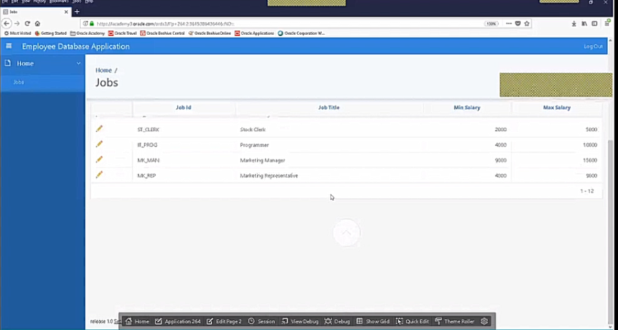
\includegraphics[width=8cm]{figure/N.png}}
            \end{figure}
\item  lalu kembali lagi kemenu sebelumnya untuk dirun aplikasinya
\begin{figure}[h]
\centerline{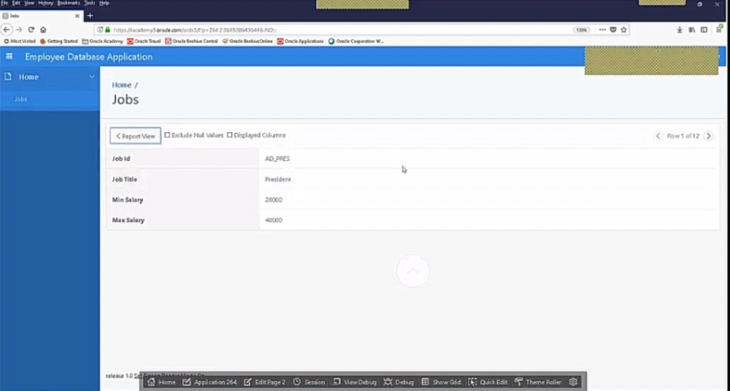
\includegraphics[width=8cm]{figure/O.png}}
            \end{figure}

\item  Lalu create  kemudian next
\begin{figure}[h]
\centerline{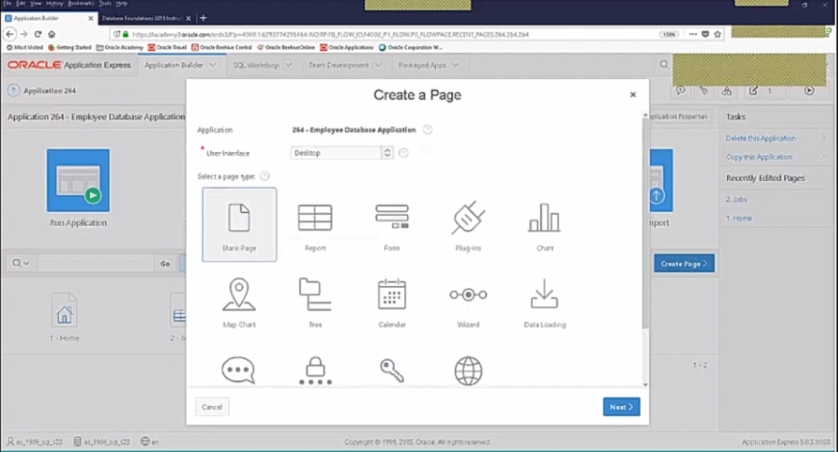
\includegraphics[width=8cm]{figure/P1.png}}
\end{figure}
\begin{figure}[h]
\centerline{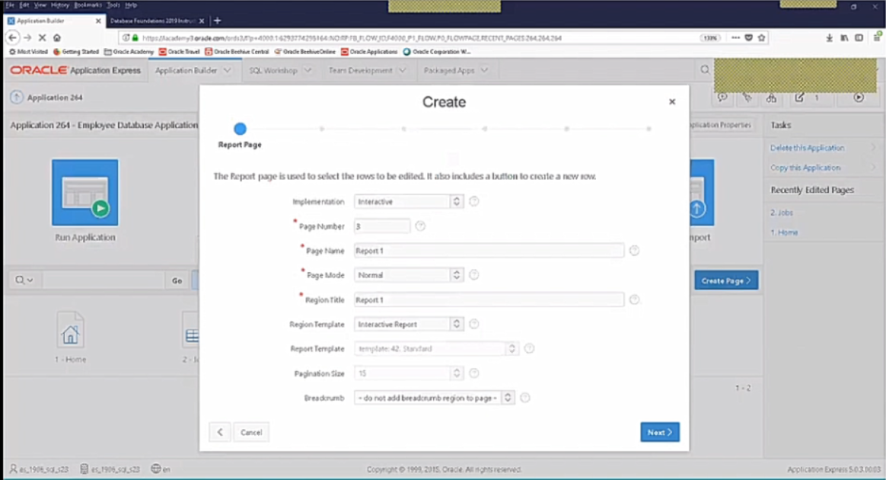
\includegraphics[width=8cm]{figure/P2.png}}
            \end{figure}
\newpage\item  Setelah itu pada step berikutnya pilih icon pencil, kemudian lanjutkan pada step 
\begin{figure}[h]
\centerline{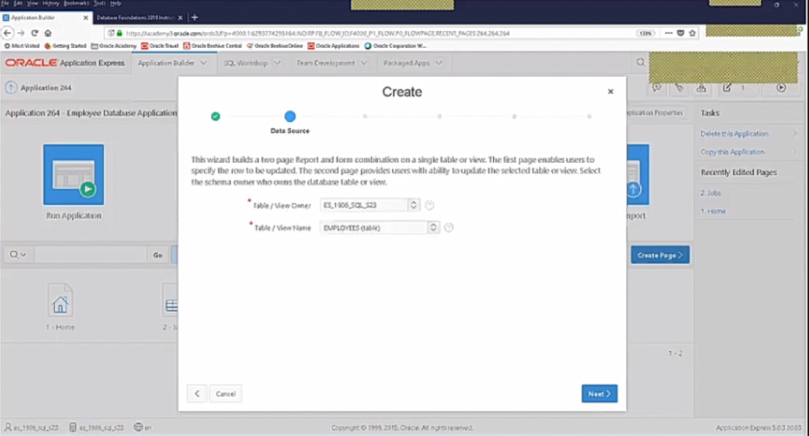
\includegraphics[width=8cm]{figure/Q1.png}}
            \end{figure}
            \begin{figure}[h]
\centerline{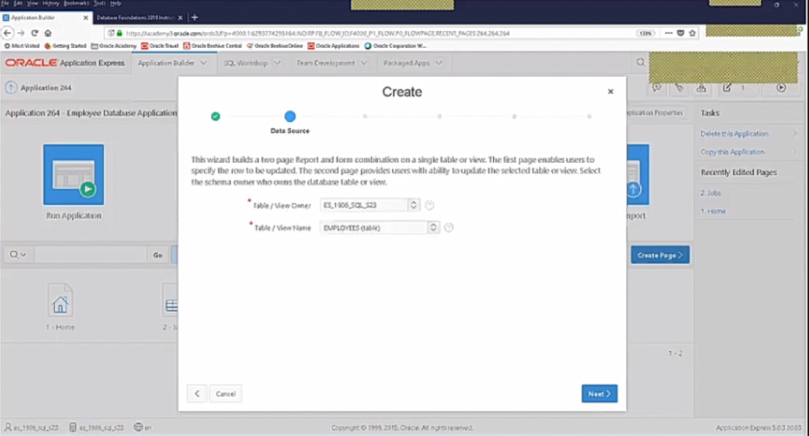
\includegraphics[width=8cm]{figure/Q1.png}}
            \end{figure}
\newpage\item  Lalu  berikutnya Jangan lupa memilih primary key agar mencegah redudansi dan tidak terjadi kekeliruan kemudian next.
\begin{figure}[h]
\centerline{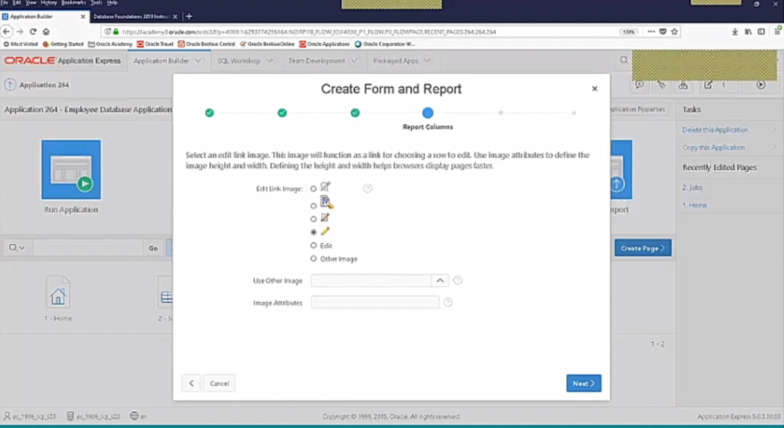
\includegraphics[width=8cm]{figure/R1.png}}
            \end{figure}
\begin{figure}[h]
\centerline{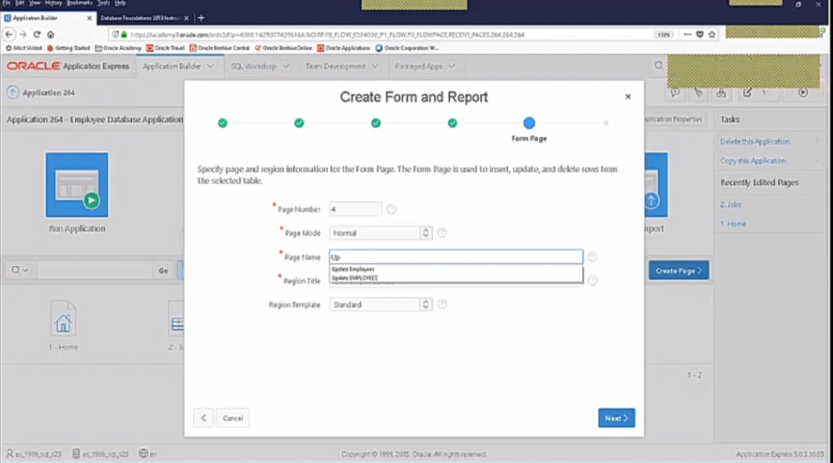
\includegraphics[width=8cm]{figure/R2.png}}
            \end{figure}
            \begin{figure}[h]
\centerline{\includegraphics[width=8cm]{figure/R3.png}}
            \end{figure}
\newpage\item  Selanjutnya next sebab data yang diinginkan telah di bentuk pada kolom disebelahnya. 
\begin{figure}[h]
\centerline{\includegraphics[width=8cm]{figure/S1.png}}
            \end{figure}
\item Selanjutnya Pembuatan dashboard ,seperti biasa membuat dashboard kemudia buka uplication yang telha dibuat, salah satunya adalah yang untuk mengupdate nya kemudian langsung buka agar bisa mengoding.
\begin{figure}[h]
\centerline{\includegraphics[width=8cm]{figure/T.png}}
            \end{figure}
\item   lalu buka halaman untuk mengoding, sebelum itu buka department id
\begin{figure}[h]
\centerline{\includegraphics[width=8cm]{figure/U2.png}}
            \end{figure}
\item   kemudian setelah terbuka dan menjoin kedua table, jangan lupa mengoding  di SQL queri untukmengecek seperti SELECT first name from employees
Jika teruning dengan baik maka berhasil.
\begin{figure}[h]
\centerline{\includegraphics[width=8cm]{figure/V.png}}
            \end{figure}
\end{enumerate}
\section{SQL Developer Data Modeler }
\subsection {Oracle SQL Developer Data Modeler menewarkan} berbagai kemampuan pemodelan data dan basis data, yang memungkinkan untuk:
\begin{enumerate}
\item Membuat  aturan dan Infoormasi bisnis
\item Membuat dan memproses Model Logical , Relational, dan Physical
\item Menyimpan informasi metadata dalam file XML
\item Menyingkron Model relasional dengan kamus data
\end{enumerate}
\subsection {Konsep Kunci:}
\begin{enumerate}

\item Membuat model logis menggunakan SQL Data 
\item Modeler Forward Engineer Model Logical ke Relational Model
\end {enumerate}

\subsection {Reverse Engineer Model Relational menerapkan standar penamaan menggunakan:}
\begin{enumerate}
\item Glosarium
\item Templete penamaan 
\end {enumerate}
\usepackage{Kesulitan: Pemula-Lokakarya ini cocok untuk seseorang yang belum pernah menggunakan Oracle SQL Developer Data Modeler tetapi  memiliki beberapa pengetahuan dasar tentang metode dan terminologi perancangan}

\subsection{Mengunduh Oracle SQL Developer Data Modeler} 
\begin{enumerate}
	\item Untuk mengunduh file instalasi, buka oracle technology network di :
http://www.oracle.com.technetwork/developer-tools/datamodeler/download/index.html
\item Pastikan anda memiliki JRE yang diinstal, jika tidak, untuh dari oracle technology network di:
http://www.oracle.com/technetwork/jave/javase/downloads/index.html

\item Buka Oracle SQL Developer Data Modeler
\item Setelah file zip Data Modeler diunduh:
\item Ekstrak file zip ke folder apa pun, didalam folder itu perluas folder data modeler
\item Klik dua kali data modeler.exe untuk 32-bit dan klik dua kali model data 64.exe untuk 64-bit
\item Referensi informasi berharga di halaman awal (Halaman ini dapat dibuka kembali dengan mengklik Bantuan , Halaman Awal)
\item Tutup Start Windows
\item Ready Go
\item Buat entitas ini dalam SQL Data Modeler
\end {enumerate}
\subsection {Kesimpulan}
Oracle SQL Data Modeler memiliki fitur-fitur canggih yang membuat  pembuatan Model Logikal dan Relasional sangat mudah dan intuitif.







\end{document}
